% ****** Start of file apssamp.tex ******
%
%   This file is part of the APS files in the REVTeX 4.2 distribution.
%   Version 4.2a of REVTeX, December 2014
%
%   Copyright (c) 2014 The American Physical Society.
%
%   See the REVTeX 4 README file for restrictions and more information.
%
% TeX'ing this file requires that you have AMS-LaTeX 2.0 installed
% as well as the rest of the prerequisites for REVTeX 4.2
%
% See the REVTeX 4 README file
% It also requires running BibTeX. The commands are as follows:
%
%  1)  latex apssamp.tex
%  2)  bibtex apssamp
%  3)  latex apssamp.tex
%  4)  latex apssamp.tex
%
\documentclass[superscriptaddress,unsortedaddress,
%runinaddress,
%frontmatterverbose, 
%preprint,
%preprintnumbers,
%nofootinbib,
%nobibnotes,
%bibnotes,
 amsmath,amssymb,
 aps,
%pra,
%prb,
%rmp,
%prstab,
%prstper,
%floatfix,
]{revtex4-2}

\usepackage{amsmath}
\usepackage{amsthm}
\usepackage{amssymb}
\usepackage[top=4cm,bottom=4cm,left=2.8cm,right=3.75cm,asymmetric,twoside]{geometry}
\usepackage{graphicx}
\usepackage{fancyhdr}
\usepackage{comment}
\usepackage{tikzorbital}
\usepackage{array} % center tables + 2 next lines
\newcolumntype{P}[1]{>{\centering\arraybackslash}p{#1}}
\newcolumntype{M}[1]{>{\centering\arraybackslash}m{#1}}
\usepackage{multirow} % confusion matrix
\newcommand\MyBox[2]{
  \fbox{\lower0.75cm
    \vbox to 2.0cm{\vfil
      \hbox to 2.0cm{\hfil\parbox{1.4cm}{#1\\#2}\hfil}
      \vfil}%
  }%
}
\usepackage{grffile}
\usepackage{epigraph} % quote
\usepackage{wrapfig} %wrapping text to fig
\usepackage{tikz} %draw figures
\usepackage{longtable}
\usepackage{subcaption} %subcaption
%\usepackage[font=small,labelfont=bf,width=0.9\textwidth]{caption}
\captionsetup[table]{skip=10pt}
\usepackage[T1]{fontenc}
%\usepackage[sc, osf]{mathpazo}
%\usepackage[euler-digits]{eulervm}
\usepackage{booktabs}
\usepackage{enumerate}
\usepackage{commath}
\usepackage{mathtools}
\usepackage[utf8]{inputenc}
\usepackage{pgfplots}
\usepgfplotslibrary{groupplots,dateplot}
\usetikzlibrary{patterns,shapes.arrows, arrows.meta,bending, shapes,calc,fadings,decorations.pathreplacing,positioning,arrows.meta}
\pgfplotsset{compat=newest}

\usepackage{sansmath}
\tikzset{>=stealth,
OptimumStyle/.style={align=center,anchor=east,rotate=90,font=\scriptsize}
}
\pgfplotsset{%samples=101,
axis lines = left,
every axis plot/.append style={line width=2pt},
}
% Include font for the identity operator
\usepackage{dsfont}
\usepackage[binary-units=true]{siunitx}
\usepackage{makecell}
\usepackage{dcolumn}% Align table columns on decimal point
\usepackage{bm}% bold math
\usepackage{physics}
\usepackage{lipsum}
\usepackage{siunitx}
\usepackage{color}
\sisetup{separate-uncertainty}
\UseRawInputEncoding
\usepackage{forest}
\forestset{
    .style={
        for tree={
            base=bottom,
            child anchor=north,
            align=center,
            s sep+=1cm,
    straight edge/.style={
        edge path={\noexpand\path[\forestoption{edge},thick,-{Latex}]
        (!u.parent anchor) -- (.child anchor);}
    },
    if n children={0}
        {tier=word, draw, thick, rectangle}
        {draw, diamond, thick, aspect=2},
    if n=1{%
        edge path={\noexpand\path[\forestoption{edge},thick,-{Latex}]
        (!u.parent anchor) -| (.child anchor) node[pos=.2, above] {Y};}
        }{
        edge path={\noexpand\path[\forestoption{edge},thick,-{Latex}]
        (!u.parent anchor) -| (.child anchor) node[pos=.2, above] {N};}
        }
        }
    }
}
\tikzset{
  green arrow/.style={
    midway,green,sloped,fill, minimum height=2cm, single arrow, single arrow head extend=.5cm, single arrow head indent=.25cm,xscale=0.3,yscale=0.15,
    allow upside down
  },
  yellow arrow/.style={
    midway,yellow,sloped,fill, minimum height=2cm, single arrow, single arrow head extend=.5cm, single arrow head indent=.25cm,xscale=0.3,yscale=0.15,
    allow upside down
  },
  black arrow/.style 2 args={-stealth, shorten >=#1, shorten <=#2},
  black arrow/.default={1mm}{1mm},
  tree box/.style={draw, rounded corners, inner sep=1em},
  node box/.style={white, draw=white, text=black, rectangle, rounded corners},
}


\newcommand{\mrk}[1]{\textcolor{red}{#1}}

\begin{document}

\title{\textit{Supplementary Information} \\ 
Predicting Solid State Material Platforms for Quantum Technologies} 

\author{Oliver Lerst{\o}l Hebnes}
\affiliation{Sopra Steria, Information Technology and Services, N-4020 Stavanger, Norway}
\affiliation{Department of Physics and Center for Computing in Science Education, University of Oslo, N-0316 Oslo, Norway}


\author{Marianne Etzelm\"uller Bathen}
\email{bathen@aps.ee.ethz.ch}
\affiliation{Advanced Power Semiconductor Laboratory, ETH Z\"urich, 8092  Z\"urich,  Switzerland} 

\author{{\O}yvind Sigmundson Sch{\o}yen}
\affiliation{Department of Physics and Center for Computing in Science Education, University of Oslo, N-0316 Oslo, Norway}

\author{Sebastian G. Winther-Larsen}
\affiliation{Menon Economics, N-0369 Oslo, Norway}
\affiliation{Department of Physics and Center for Computing in Science Education, University of Oslo, N-0316 Oslo, Norway}

\author{Lasse Vines}
\affiliation{Department of Physics and Center for Materials Science and Nanotechnology, University of Oslo, N-0316 Oslo, Norway}

\author{Morten Hjorth-Jensen}
\affiliation{Department of Physics and Astronomy and Facility for Rare Ion Beams, Michigan State University, East Lansing, MI 48824, USA}
\affiliation{Department of Physics and Center for Computing in Science Education, University of Oslo, N-0316 Oslo, Norway}

\pacs{02.70.Ss, 31.15.A-, 31.15.bw, 71.15.-m, 73.21.La}

\maketitle


\noindent \textbf{Contents:} 
\begin{itemize}
    \item \textit{Supplementary methods.} \\   Additional information on the featurization process and optimization of the machine learning methods. 
    \item \textit{Supplementary results.} \\ Statistics and tables over the materials that were predicted by the machine learning methods based on the labeled data sets derived using the three different data mining approaches. The supplementary results also include feature analyses for the materials predicted by the machine learning methods as suitable for QT. 
    \item \textit{Supplementary references.}  
\end{itemize}

\newpage 

\section*{Supplementary methodology}
\subsection*{Featurization}
To apply Matminer's featurization tools, we extend an existing implementation by \citeauthor{Breuck2021} \cite{Breuck2021}. 
Table~\ref{table:featurizers} contains an overview of the 39  chosen featurizers from Matminer. The featurization process results in $4876$ physics informed descriptors. 

The motivation behind the choice of featurizers is that we do not precisely know which features describe a suitable quantum host material.  Therefore, we have collected a large quantity of descriptors in order to reliably  predict potential materials for quantum technologies. 


\begin{center}
\begin{longtable}{M{3.5cm} M{6.5cm} M{2.0cm}}
\caption{Descriptions of the 39 featurizers from Matminer that have been emplyed in this work. Descriptions are either found from Ref. \cite{Ward2018} or from the project's Github page. For entries lacking references, we refer to Ref.~\cite{Ward2018}.}
\label{table:featurizers} 
\\ \hline
Features & Description & Reference \\
\hline 
  \textbf{Composition features} & & \\ 
  AtomicOrbitals & Highest occupied molecular orbital (HOMO) & \cite{Kotochigova1997}  \\   
   & and lowest unoccupied molecular orbital (LUMO) &  \\   
  AtomicPacking-Efficiency & Packing efficiency & \cite{Laws2015}  \\   
  BandCenter & Estimate absolute position of band center  & \cite{Butler1978} \\   
   & using geometric mean of electronegativity &  \\  
  ElementFraction & Fraction of each element in a composition &    \\   
  ElementProperty & Statistics of various element properties & \cite{Ong2013,Ward2016, Deml2016}  \\   
  IonProperty & Maximum and average ionic character & \cite{Ward2016} \\   
  Miedema & Formation enthalpies of intermetallic compounds, solid solutions, & \cite{Weeber1987} \\   
   & and amorphous phases using semi-empirical Miedema model &  \\   
  Stoichiometry & $L^p$ norm-based stoichiometric attributes & \cite{Ward2016} \\   
  TMetalFraction & Fraction of magnetic transition metals & \cite{Deml2016}  \\   
  ValenceOrbital & Valence orbital attributes such as & \cite{Ward2016}  \\   
   &  the mean number of electrons in each shell &   \\   
  YangSolid-Solution & Mixing thermochemistry and size mismatch terms & \cite{Yang2012} \\
    \hline 
  \textbf{Oxide composition features} &  &  \\
  Electronegativity-Diff & Statistics on electronegativity difference & \cite{Deml2016} \\   
   &  between anions and cations & \\ 
  OxidationStates & Statistics of oxidation states & \cite{Deml2016}  \\   
\hline 
  \textbf{Structure features} & & \\   
  DensityFeatures & Calculate density, volume per atom and packing fraction & - \\   
  GlobalSymmetry-Features & Determines spacegroup number, crystal system  & - \\   
   & (1-7) and inversion symmetry & \\ 
  RadialDistribution-Function & Calculates the radial distribution  & - \\   
   & function of a crystal system & \\ 
  CoulombMatrix & Generate the Coulomb matrix for nuclear interactions  & \cite{Rupp2012}  \\    
  %CoulombMatrix & Generate the Coulomb matrix, which is a representation of the nuclear coulombic interaction of the input structure. & \cite{Rupp2012}  \\      
  PartialRadial-Distribution-Function & Compute the partial radial distribution  & \cite{Schuett2014}  \\   
   & function of a crystal structure & \\ 
  SineCoulomb-Matrix & Computes a variant of the coulomb matrix & \cite{Faber2015}  \\   
   & developed for periodic crystals & \\ 
  EwaldEnergy & Computes the energy from Coulombic interactions  & \cite{Ewald1921}  \\   
   & based on charge states of each site & \\ 
  BondFractions & Compute the fraction of each bond in a  & \cite{Hansen2015}  \\   
   & structure, based on nearest neighbors & \\ 
  Structural Heterogeneity & Calculates the variance in bond lengths and  & \cite{Ward2017}  \\   
   & atomic volumes in a structure & \\ 
  MaximumPacking-Efficiency & Calculates the maximum packing efficiency of a structure & \cite{Ward2017} \\   
  Chemical-Ordering & Computes how much the ordering of species  & \cite{Ward2017}  \\   
   & differs from random in a structure & \\ 
  XRDPowder-Pattern & 1D array representing normalized powder diffraction & \cite{Ong2013} \\ 
   &of a structure as calculated by pymatgen  & \\ 
    \hline 
  \textbf{Site features} & & \\
  AGNI-Fingerprints & Calculates the product integral of RDF & \cite{Botu2014}  \\    
   & and Gaussian window function  & \\ 
  AverageBond- Agle & Determines the average bond angle of a specific  & \cite{Jong2016}  \\
   & site with its nearest neighbors  & \\ 
  AverageBond-Length & Determines the average bond length between one specific site & \cite{Jong2016}  \\ 
   & and all its nearest neighbors  & \\ 
  BondOrientational-Parameter & Calculates the averages of spherical  & \cite{Seko2017, Steinhardt1983}  \\ 
   & harmonics of local neighbors & \\ 
  ChemEnvSite-Fingerprint & Calculates the resemblance of given sites to ideal & \cite{Waroquiers2017, Zimmermann2017}  \\   
   & environment using pymatgens ChemEnv package  & \\ 
  Coordination-Number & The number of first nearest neighbors of a site & \cite{Zimmermann2017}  \\
  CrystalNN-Fingerprint & A local order parameter fingerprint for periodic crystals & -  \\   
  GaussianSymm-Func & Calculates the gaussian radial and angular symmetry functions  & \cite{Behler2011,Khorshidi2016}  \\   
   & originally suggested for fitting machine learning potentials &  \\ 
  GeneralizedRadial-Distribution-Function & Computes the general radial distribution function for a site & \cite{Seko2017}  \\   
  LocalProperty-Difference & Computes the difference in elemental properties  & \cite{Ward2017, Jong2016} \\   
   & between a site and its neighboring sites & \\ 
  OPSite-Fingerprint & Computes the local structure order parameters & \cite{Zimmermann2017} \\   
   & from a site's neighbor environment  & \\ 
  Voronoi-Fingerprint & Calculates the Voronoi tessellation-based  & \cite{Peng2011,Wang2019} \\
   & features around a target site & \\ 
\hline     
  \textbf{Density of state features} & & \\
  DOSFeaturizer & Computes top contributors to the density of  & \cite{Dylla2020} \\ 
  & states at the VBM and CBM  & \\ 
  %DOSFeaturizer & Computes top contributors to the density of states at the valence and conduction band edges. Thus includes chemical species, orbital character, and orbital location information. & \cite{Dylla2020} \\
  \hline  
  \textbf{Band structure features} & & \\
  BandFeaturizer & Converts a complex electronic band  & - \\ 
   &structure into discrete quantities  & \\ 
%BandFeaturizer & Converts a complex electronic band structure into quantities such as band gap and the norm of k point coordinates at which the conduction band minimum and valence band maximum occur. & - \\
\hline 
\end{longtable}
\end{center}


\subsection*{\mrk{Data mining: The extended Ferrenti approach}} 

\mrk{This section contains the findings from the data mining and feature analysis for the extended Ferrenti approach to complement the discussion in the main text on the Ferrenti and empirical approaches.}  

\mrk{In the labeled dataset of the extended Ferrenti approach, we find a single entry for each of SiC, Si, GaN, ZnS, GaP, AlAs and AlP, carbon in both diamond- and graphite-like structures, and AlN in three different configurations. The labeled dataset includes a larger variety of materials that are known to be quantum compatible as compared to the Ferrenti approach due to admitting more elements in the initial selection process. However, since we also included a more stringent band gap restriction of $1.5$~eV (to reduce the amount of materials in the training set), there is a more sparse representation of each known chemical formula present in the labeled data. }

\mrk{Figure~\ref{fig:parallel-coordinates-approaches} displays the parallel coordinate plot for the extended Ferrenti approach while Figure~\ref{fig:2dscatterplotpca} contains the two-dimensional scatter plot for the same approach. The qualitative behavior of the data set derived during the data mining of the extended Ferrenti approach can be seen to overlap with that of the Ferrenti approach. }

\begin{figure}[t] %!htp
    \centering
    \begin{subfigure}{1\textwidth}
        \centering
          \scalebox{0.85}{\input{figures/parallel-coordinates-plots/02-extended-ferrenti-approach-v3.pgf}}
    \end{subfigure}
    \caption{\mrk{Parallel coordinate plot for the extended Ferrenti approach. To limit data cluttering, we have randomly collected up to $250$ entries for each class. The axes show total magnetization (mag), space group (SG), ionic character (ionic char), covalent range (cov range) as calculated from elemental properties, number of elements (num elements) and energy gap (Eg) as extracted from the MP database.}} 
    \label{fig:parallel-coordinates-approaches}
\end{figure}

\begin{figure}%[h] %!tbp
    \centering
    \begin{subfigure}{0.5\textwidth}
        \centering
        \includegraphics[width=1\textwidth]{figures/pca-2d-plots/02-augmented-ferrenti-approach.pdf}
    \end{subfigure}
    \caption{\mrk{Two-dimensional scatter plot for the extended Ferrenti approach. We have identified the eigenvectors corresponding to the two largest eigenvalues of the covariance-matrix, that is, the two most important principal components of the initial data from the Materials Project query. Then, we have transformed the sets of labeled data resulting from the three approaches and visualized them as scatter plots. Green squares display suitable candidates and red triangles represent unsuitable candidates.}}
    \label{fig:2dscatterplotpca}
\end{figure}

\subsection*{Optimization of machine learning methods}

In the evaluation of the machine learning methods for the three different approaches, we apply a $5\times 5$ stratified cross-validation when searching for the optimal hyperparameter combinations, see for example Ref.~\cite{Hastie2009} for details on the cross-validation procedure. We apply four different evaluation metrics to each of the four machine learning algorithms discussed in this work. 

The implementation of the machine learning methods was achieved through the machine learning library Scikit-Learn \cite{Pedregosa2012}. Adjusting many of the hyperparameters in Scikit-Learn resulted in severe overfitting for the machine learning methods random forests, gradient boosting, and decision trees. Therefore, most parameters are the default values defined by Scikit-Learn. The only parameter that was found to potentially improve the evaluation metric F$1$  (see Refs.~\cite{sammut2010,geron2022} for a definition of various metrics) was the maximum depth for the decision trees (these are also used as so-called weak learners in ensemble methods like gradient boosting and random forests \cite{geron2022}). In our work we adjusted 
the depth of the trees to vary from $1$ to $8$. For logistic regression, we chose to adjust the regularization strength with seven logarithmic values ranging from $10^{-3}$ to $10^{5}$, and used either $200$ or $400$ iterations to reach convergence. 

When searching for the optimal number of principal components, we iterated over every odd number of principal components from $1$ to the upper restricted number which defines an accumulated variance of $95 \ \%$ from the principal component analysis. Due to a large number of principal components, we performed a fit of  $25$ folds for each of the $1232$ parameter combinations, totaling up to $30,800$ individual models. 


\subsubsection*{Ferrenti approach}
The grid search for the optimal number of principal components for the Ferrenti approach is visualized in Fig.~\ref{fig:01-pca}, where we present the mean accuracy of the four ML models applied to the training set, and the balanced accuracy, precision, recall, and F$1$-score 
for the test set as a function of the number of principal components. For each principal component, we display the optimal combination of  hyperparameters based on the F$1$-score. 

\begin{figure}[ht!]
\begin{subfigure}[b]{1.0\textwidth}
    \centering
    % This file was created by tikzplotlib v0.9.8.
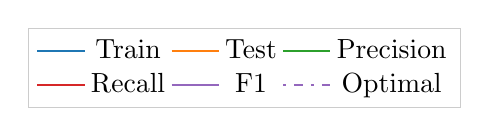
\begin{tikzpicture}

\definecolor{color0}{rgb}{0.12156862745098,0.466666666666667,0.705882352941177}
\definecolor{color1}{rgb}{1,0.498039215686275,0.0549019607843137}
\definecolor{color2}{rgb}{0.172549019607843,0.627450980392157,0.172549019607843}
\definecolor{color3}{rgb}{0.83921568627451,0.152941176470588,0.156862745098039}
\definecolor{color4}{rgb}{0.580392156862745,0.403921568627451,0.741176470588235}
\begin{axis}[%
 hide axis,
 xmin=10,
 xmax=50,
 ymin=0,
 ymax=0.4,
 legend columns=3,
 legend style={
   fill opacity=1,
   draw opacity=1,
   text opacity=1,
   align=center,
   anchor=north,
   draw=white!80!black
 },
 ]
 \addlegendimage{semithick, color0}
 \addlegendentry{Train};
 \addlegendimage{semithick, color1}
 \addlegendentry{Test};
 \addlegendimage{semithick, color2}
 \addlegendentry{Precision};
 \addlegendimage{semithick, color3}
 \addlegendentry{Recall};
 \addlegendimage{semithick, color4}
 \addlegendentry{F1};
 \addlegendimage{semithick, color4, dash pattern=on 1pt off 3pt on 3pt off 3pt}
 \addlegendentry{Optimal};
 \end{axis}

\end{tikzpicture}

  \end{subfigure}
  \par\bigskip
  \begin{subfigure}[b]{0.5\textwidth}
    \input{figures/optimizing-parameters/01-ferrenti-approach-176-LOG}
    \caption{}
    \label{fig:q1-LOG}
  \end{subfigure}%
    \hfill
  \begin{subfigure}[b]{0.5\textwidth}
    \input{figures/optimizing-parameters/01-ferrenti-approach-176-DT}
    \caption{}
    \label{fig:q1-DT}
  \end{subfigure}
  \begin{subfigure}[b]{0.5\textwidth}
    \input{figures/optimizing-parameters/01-ferrenti-approach-176-RF.tex}
    \caption{}
    \label{fig:q1-RF}
  \end{subfigure}%
   \hfill
  \begin{subfigure}[b]{0.5\textwidth}
    \input{figures/optimizing-parameters/01-ferrenti-approach-176-GB.tex}
    \caption{}
    \label{fig:q1-GB}
  \end{subfigure}
  \caption{Four figures displaying hyperparameter search for the Ferrenti approach. The best estimator is visualized for all hyperparameters as a function of principal components during a grid search with a $5\times5$ stratified cross-validation. The dotted lines mark the optimal hyperparameter-combination. Train stands for normal training accuracy, while test is the balanced accuracy on the test set. Precision, recall, and F$1$ scores are based on the test set. The number of principal components that explain the $95 \ \%$ accumulated variance is $144$, while the optimal model is found using the F$1$-score.}
  \label{fig:01-pca}
\end{figure}

\begin{table}[b]
\centering
\caption{Optimal number of principal components and the respective scores (standard deviation) for each of the four ML methods logistic regression (LOG), decision trees (DT), random forests (RF) and gradient boosting (GB) in the Ferrenti approach, as visualized by the dash-dotted line in Fig.~\ref{fig:01-pca}.}
\label{tab:01-pc}
\noindent\makebox[\textwidth]{
\begin{tabular}{M{2.0cm} M{1.5cm} M{2.0cm} M{2.0cm}M{2.0cm}M{2.0cm} }
  \hline
  \hline
   Method & PC & Mean test & Mean precision & Mean recall & mean F1\\
  \hline
  LOG & $171$ & $0.98(0.012)$ & $0.98(0.011)$ & $0.99(0.007)$ & $0.99(0.007)$ \\
  DT & $37$   & $0.77(0.034)$ & $0.84(0.034)$ & $0.85(0.044)$ & $0.84(0.022)$ \\
  RF & $53$   & $0.87(0.027)$ & $0.88(0.022)$ & $0.98(0.010)$ & $0.93(0.014)$ \\
  GB & $107$  & $0.92(0.016)$ & $0.92(0.015)$ & $0.98(0.010)$ & $0.95(0.009)$ \\
  \hline
\end{tabular}
}
\end{table}

In Table~\ref{tab:01-pc}, we include the precise measurements for each of the evaluation metrics for the optimal number of principal components. The optimal number is visualized as dotted lines in Fig.~\ref{fig:01-pca}. The relevant hyperparameters for logistic regression were the maximum iterations. The number of iterations was set to $400$, and the optimal regularization term was $0.46$. For random forests and decision trees, we found the maximum depth to be $7$. Gradient boosting, which normally uses a weak learner, had a decision tree depth of $4$. We found the best performing method to be logistic regression, but this method depends on a large number of principal components. 

In Fig.~\ref{fig:01-fi}, we visualize how the various machine learning methods  interpret the principal components that are sorted in descending order by the explained variance, found through a $5\times 5$ stratified cross-validation approach. To reach the $95 \ \%$ accumulated explained variance, a total of $144$ principal components were included. We have visualized the first $25$ components since these capture the most important information. We note that most of the important features are found within the first five principal components.

\begin{figure}[ht!]
  \begin{subfigure}[b]{0.5\textwidth}
    \centering
    \input{figures/feature-importance/01-ferrenti-approachLOG-final.tex}
    \label{fig:01-fi-a}
  \end{subfigure}%

  \begin{subfigure}[b]{0.5\textwidth}
    \centering
    \input{figures/feature-importance/01-ferrenti-approachDT-final.tex}
    \label{fig:01-fi-b}
  \end{subfigure}%

  \begin{subfigure}[b]{0.5\textwidth}
    \centering
    \input{figures/feature-importance/01-ferrenti-approachRF-final.tex}
    \label{fig:01-fi-c}
  \end{subfigure}%

  \begin{subfigure}[b]{0.5\textwidth}
    \centering
    \input{figures/feature-importance/01-ferrenti-approachGB-final.tex}
    \label{fig:01-fi-d}
  \end{subfigure}%

  \begin{subfigure}[b]{0.5\textwidth}
    \centering
    % This file was created by tikzplotlib v0.9.8.
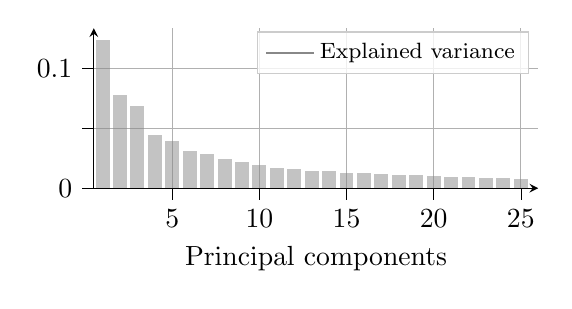
\begin{tikzpicture}

\definecolor{color0}{rgb}{0.8,0.4,0.466666666666667}

\begin{axis}[
height=1.4222438079424382in,
legend style={fill opacity=0.8, draw opacity=1, text opacity=1, draw=white!80!black},
tick align=outside,
tick pos=left,
width=2.8444876158848764in,
x grid style={white!69.0196078431373!black},
xlabel={Principal components},
xmajorgrids,
xmin=0.5, xmax=26,
xtick style={color=black},
y grid style={white!69.0196078431373!black},
ymajorgrids,
ymin=0, ymax=0.133808014644924,
ytick style={color=black},
yticklabels={, 0, , 0.1},
legend style={font=\footnotesize},
]
\draw[draw=none,fill=white!53.3333333333333!black,fill opacity=0.5] (axis cs:0.6,0) rectangle (axis cs:1.4,0.123808014644924);
\draw[draw=none,fill=white!53.3333333333333!black,fill opacity=0.5] (axis cs:1.6,0) rectangle (axis cs:2.4,0.0779020383908885);
\draw[draw=none,fill=white!53.3333333333333!black,fill opacity=0.5] (axis cs:2.6,0) rectangle (axis cs:3.4,0.0690715494994265);
\draw[draw=none,fill=white!53.3333333333333!black,fill opacity=0.5] (axis cs:3.6,0) rectangle (axis cs:4.4,0.0448634890553009);
\draw[draw=none,fill=white!53.3333333333333!black,fill opacity=0.5] (axis cs:4.6,0) rectangle (axis cs:5.4,0.0396017649392185);
\draw[draw=none,fill=white!53.3333333333333!black,fill opacity=0.5] (axis cs:5.6,0) rectangle (axis cs:6.4,0.0309892340254588);
\draw[draw=none,fill=white!53.3333333333333!black,fill opacity=0.5] (axis cs:6.6,0) rectangle (axis cs:7.4,0.0286471759268761);
\draw[draw=none,fill=white!53.3333333333333!black,fill opacity=0.5] (axis cs:7.6,0) rectangle (axis cs:8.4,0.0241373022722755);
\draw[draw=none,fill=white!53.3333333333333!black,fill opacity=0.5] (axis cs:8.6,0) rectangle (axis cs:9.4,0.0219387724823991);
\draw[draw=none,fill=white!53.3333333333333!black,fill opacity=0.5] (axis cs:9.6,0) rectangle (axis cs:10.4,0.0191941500093896);
\draw[draw=none,fill=white!53.3333333333333!black,fill opacity=0.5] (axis cs:10.6,0) rectangle (axis cs:11.4,0.0170987447716404);
\draw[draw=none,fill=white!53.3333333333333!black,fill opacity=0.5] (axis cs:11.6,0) rectangle (axis cs:12.4,0.0163324377943715);
\draw[draw=none,fill=white!53.3333333333333!black,fill opacity=0.5] (axis cs:12.6,0) rectangle (axis cs:13.4,0.0142479118996461);
\draw[draw=none,fill=white!53.3333333333333!black,fill opacity=0.5] (axis cs:13.6,0) rectangle (axis cs:14.4,0.0139471831901937);
\draw[draw=none,fill=white!53.3333333333333!black,fill opacity=0.5] (axis cs:14.6,0) rectangle (axis cs:15.4,0.0125561362477749);
\draw[draw=none,fill=white!53.3333333333333!black,fill opacity=0.5] (axis cs:15.6,0) rectangle (axis cs:16.4,0.0122752355665442);
\draw[draw=none,fill=white!53.3333333333333!black,fill opacity=0.5] (axis cs:16.6,0) rectangle (axis cs:17.4,0.0117377683648439);
\draw[draw=none,fill=white!53.3333333333333!black,fill opacity=0.5] (axis cs:17.6,0) rectangle (axis cs:18.4,0.0108124054147357);
\draw[draw=none,fill=white!53.3333333333333!black,fill opacity=0.5] (axis cs:18.6,0) rectangle (axis cs:19.4,0.0105912984624588);
\draw[draw=none,fill=white!53.3333333333333!black,fill opacity=0.5] (axis cs:19.6,0) rectangle (axis cs:20.4,0.00987028371434172);
\draw[draw=none,fill=white!53.3333333333333!black,fill opacity=0.5] (axis cs:20.6,0) rectangle (axis cs:21.4,0.00946157777094173);
\draw[draw=none,fill=white!53.3333333333333!black,fill opacity=0.5] (axis cs:21.6,0) rectangle (axis cs:22.4,0.00932051055389097);
\draw[draw=none,fill=white!53.3333333333333!black,fill opacity=0.5] (axis cs:22.6,0) rectangle (axis cs:23.4,0.00851928669553865);
\draw[draw=none,fill=white!53.3333333333333!black,fill opacity=0.5] (axis cs:23.6,0) rectangle (axis cs:24.4,0.00821174057436937);
\draw[draw=none,fill=white!53.3333333333333!black,fill opacity=0.5] (axis cs:24.6,0) rectangle (axis cs:25.4,0.00796122578616887);
\addlegendimage{semithick, color=white!53.3333333333333!black};
\addlegendentry{Explained variance};
\end{axis}

\end{tikzpicture}

    \label{fig:01-fi-e}
  \end{subfigure}%

  \caption{Visualization of different parameters for the $25$ most principal components ranked in descending order by the explained variance for the Ferrenti approach. The panels show the logistic regression coefficients, decision trees feature importance, random forests feature importance, gradient boosting feature importance, and explained variance that is retained by choosing each of the eigenvectors. }
  \label{fig:01-fi}
\end{figure}


For logistic regression, we have visualized the mean fitted coefficients and the standard deviation in the top panel of Fig.~\ref{fig:01-fi}. Large positive or negative coefficients can be considered increasingly important, where positive (negative) coefficients will contribute to making positive (negative) predictions. In the next three panels we visualize the mean impurity-based feature importance and the standard deviation for the ML methods decision trees, random forests, and gradient boosting, respectively. We observe that the single most important feature for all ML methods in the Ferrenti approach is the fifth principal component. Selecting the highest values of this eigenvector, we find that the corresponding features originate from the DFT band gap of the elemental solids among the elements in the compound as calculated by Materials Agnostic Platform for Informatics and Exploration (MagPie). 

After the first ten principal components, we observe that the methods adapt the other principal components with varying degrees. The coefficients for the case of logistic regression experience large fluctuations, but the three remaining models find that the first and second principal components are important in addition to the fifth. In order of importance, we observe that the second component's largest values correspond to the electronegativity, maximum ionic character, and covalent radius among the elements in the composition. The data originates from elemental calculations from MagPie and are aggregated as either minimum, mean, standard deviation, or maximum. While the first principal component encompasses the largest explained variance, it does not provide any specific information on which features it represents.


\subsubsection*{Extended Ferrenti approach}

\begin{figure}[ht!]
  \begin{subfigure}[b]{1.0\textwidth}
    \centering
    % This file was created by tikzplotlib v0.9.8.
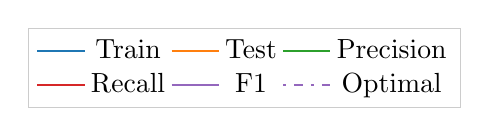
\begin{tikzpicture}

\definecolor{color0}{rgb}{0.12156862745098,0.466666666666667,0.705882352941177}
\definecolor{color1}{rgb}{1,0.498039215686275,0.0549019607843137}
\definecolor{color2}{rgb}{0.172549019607843,0.627450980392157,0.172549019607843}
\definecolor{color3}{rgb}{0.83921568627451,0.152941176470588,0.156862745098039}
\definecolor{color4}{rgb}{0.580392156862745,0.403921568627451,0.741176470588235}
\begin{axis}[%
 hide axis,
 xmin=10,
 xmax=50,
 ymin=0,
 ymax=0.4,
 legend columns=3,
 legend style={
   fill opacity=1,
   draw opacity=1,
   text opacity=1,
   align=center,
   anchor=north,
   draw=white!80!black
 },
 ]
 \addlegendimage{semithick, color0}
 \addlegendentry{Train};
 \addlegendimage{semithick, color1}
 \addlegendentry{Test};
 \addlegendimage{semithick, color2}
 \addlegendentry{Precision};
 \addlegendimage{semithick, color3}
 \addlegendentry{Recall};
 \addlegendimage{semithick, color4}
 \addlegendentry{F1};
 \addlegendimage{semithick, color4, dash pattern=on 1pt off 3pt on 3pt off 3pt}
 \addlegendentry{Optimal};
 \end{axis}

\end{tikzpicture}

  \end{subfigure}
\par\bigskip
  \begin{subfigure}[b]{0.5\textwidth}
    \input{figures/optimizing-parameters/02-augmented-ferrenti-approach-176-LOG.tex}
    \caption{}
    \label{fig:q2-LOG}
  \end{subfigure}%
  \hfill
  \begin{subfigure}[b]{0.5\textwidth}
    \input{figures/optimizing-parameters/02-augmented-ferrenti-approach-176-DT.tex}
    \caption{}
    \label{fig:q2-DT}
  \end{subfigure}

  \begin{subfigure}[b]{0.5\textwidth}
    \input{figures/optimizing-parameters/02-augmented-ferrenti-approach-176-RF.tex}
    \caption{}
    \label{fig:q2-RF}
  \end{subfigure}%
  \hfill
  \begin{subfigure}[b]{0.5\textwidth}
    \input{figures/optimizing-parameters/02-augmented-ferrenti-approach-176-GB.tex}
    \caption{}
    \label{fig:q2-GB}
  \end{subfigure}
  \caption{Hyperparameter search for the extended Ferrenti approach. The best estimator is visualized for all hyperparameters as a function of principal components during a grid search with a $5\times5$ stratified cross-validation, and the dotted lines mark the optimal hyperparameter combination. Train stands for normal training accuracy, while test is the balanced accuracy on the test set. Precision, recall and F$1$ scores  are based on the test set. The number of principal components that explain the $95 \ \%$ accumulated variance is $159$, while the optimal model is found using the F$1$-score.}
  \label{fig:02-pca}
\end{figure}

For the extended Ferrenti approach, the parameter grid search for principal components is visualized in Figure~\ref{fig:02-pca}. All methods experience an almost perfect recall score for the first principal component due to the largely imbalanced dataset with $2141$ suitable and $684$ unsuitable candidates, which results in  a ratio of $75 \ \% : 25 \ \%$ (suitable:unsuitable). This ratio comes as a consequence of the ML methods being able to correctly label many suitable candidates compared to the number of unsuitable candidates. 
On the other hand, we find a low precision score for the first component since the ML methods  predict many materials as suitable regardless of whether they were labeled as suitable or unsuitable in the initial data labeling process. 
This trend is revealed when looking at the balanced accuracy score. For all figures, it remains the lowest score of the evaluation metrics largely due to the inaccuracy of true negatives for the cross-validations.  


Overall the search for optimal hyperparameters in Fig.~\ref{fig:02-pca} for the extended Ferrenti approach bears resemblance to Fig.~\ref{fig:01-pca} for the Ferrenti approach. Logistic regression performs optimally for many principal components, and is the only method that continues to improve with an increasing number of components. The decision trees method exhibits a large fluctuation of scores, where the number of false positives is dominating the balanced accuracy score. The random forests method exhibits fewer fluctuations compared to decision trees as a consequence of the ensemble decision trees, while gradient boosting does not improve beyond $100$ principal components.

\begin{table}[t]
\centering
\caption{Optimal number of principal components and the respective scores (standard deviation) for each of the four ML methods logistic regression (LOG), decision trees (DT), random forests (RF) and gradient boosting (GB) in the extended Ferrenti approach, as visualized by the dash-dotted line in Fig.~\ref{fig:02-pca}.}
\label{tab:02-pc}
\noindent\makebox[\textwidth]{
\begin{tabular}{M{2.0cm} M{1.5cm} M{2.0cm} M{2.0cm}M{2.0cm}M{2.0cm} }
  \hline
  \hline
   Method & PC & Mean test &  Mean precision & Mean recall & mean F1\\
  \hline
  LOG & $175$ & $0.98(0.008)$ & $0.99(0.004)$ & $0.99(0.004)$ & $0.99(0.003)$ \\
  DT & $25$   & $0.69(0.034)$ & $0.86(0.015)$ & $0.93(0.021)$ & $0.90(0.008)$ \\
  RF & $25$   & $0.70(0.028)$ & $0.86(0.011)$ & $1.00(0.003)$ & $0.93(0.006)$ \\
  GB & $93$   & $0.85(0.025)$ & $0.93(0.011)$ & $0.99(0.004)$ & $0.96(0.007)$ \\
  \hline
\end{tabular}
}
\end{table}

The optimal hyperparameters for the extended Ferrenti approach are summarized in Table~\ref{tab:02-pc}. We find that logistic regression with $175$ principal components performs more or less like a perfect classifier with overall high scores. The decision trees and random forests methods have similar balanced accuracy scores with $0.69$ and $0.70$, respectively, due to challenges associated with predicting true negative labels for $25$ principal components. Lastly, we find that gradient boosting performs optimally at $93$ principal components with a balanced accuracy score of $0.85$. 

The relevant hyperparameters for logistic regression are the regularization strength and the maximum iterations, which were set to $0.46$ and $400$, respectively. Smaller regularization values resulted in worse scores, while increasing values did not noticeably affect the results. The decision trees and random forests methods both found an optimal maximum depth of seven, where smaller values resulted in low precision but high recall.  Therefore, the choice was made to facilitate a compromise between precision and recall. For gradient boosting, we find the optimal maximum depth to be four due to a decline in overall metrics for increasing depth.
That is, except for the training accuracy, demonstrating a case of potential overfitting.


The interpretation of feature importance for the extended Ferrenti approach is substantially more difficult than in the Ferrenti approach. We find for logistic regression and decision trees that no feature is different than any other in the cross-validation due to a large variety of accuracy. However, we find that random forests and gradient boosting experience the fifth principal component as important. 
Similar to the Ferrenti approach, the extended Ferrenti approach finds the DFT band gap of the elemental solids among the elements in the composition to be important. The feature regarding the band gap originates from the highest value from the first principal component. 
This means that, if we consider, e.g., the compound SiC, the band gaps of both SiC, Si and C would be considered important by the ML methods. 

\subsubsection*{Empirical approach}

\begin{figure}[ht!]
  \begin{subfigure}[b]{1.0\textwidth}
    \centering
    % This file was created by tikzplotlib v0.9.8.
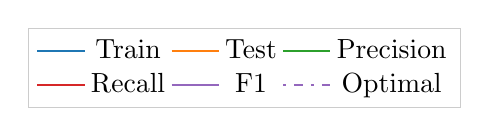
\begin{tikzpicture}

\definecolor{color0}{rgb}{0.12156862745098,0.466666666666667,0.705882352941177}
\definecolor{color1}{rgb}{1,0.498039215686275,0.0549019607843137}
\definecolor{color2}{rgb}{0.172549019607843,0.627450980392157,0.172549019607843}
\definecolor{color3}{rgb}{0.83921568627451,0.152941176470588,0.156862745098039}
\definecolor{color4}{rgb}{0.580392156862745,0.403921568627451,0.741176470588235}
\begin{axis}[%
 hide axis,
 xmin=10,
 xmax=50,
 ymin=0,
 ymax=0.4,
 legend columns=3,
 legend style={
   fill opacity=1,
   draw opacity=1,
   text opacity=1,
   align=center,
   anchor=north,
   draw=white!80!black
 },
 ]
 \addlegendimage{semithick, color0}
 \addlegendentry{Train};
 \addlegendimage{semithick, color1}
 \addlegendentry{Test};
 \addlegendimage{semithick, color2}
 \addlegendentry{Precision};
 \addlegendimage{semithick, color3}
 \addlegendentry{Recall};
 \addlegendimage{semithick, color4}
 \addlegendentry{F1};
 \addlegendimage{semithick, color4, dash pattern=on 1pt off 3pt on 3pt off 3pt}
 \addlegendentry{Optimal};
 \end{axis}

\end{tikzpicture}

  \end{subfigure}
  \par\bigskip
  \begin{subfigure}[b]{0.5\textwidth}
    \input{figures/optimizing-parameters/03-insightful-approach-176-LOG.tex}
    \caption{}
    \label{fig:q3-LOG}
  \end{subfigure}%
  \hfill
  \begin{subfigure}[b]{0.5\textwidth}
    \input{figures/optimizing-parameters/03-insightful-approach-176-DT.tex}
    \caption{}
    \label{fig:q3-DT}
  \end{subfigure}
  \begin{subfigure}[b]{0.5\textwidth}
    \input{figures/optimizing-parameters/03-insightful-approach-176-RF.tex}
    \caption{}
    \label{fig:q3-RF}
  \end{subfigure}%
  \hfill
  \begin{subfigure}[b]{0.5\textwidth}
    \input{figures/optimizing-parameters/03-insightful-approach-176-GB.tex}
    \caption{}
    \label{fig:q3-GB}
  \end{subfigure}

  \caption{{Hyperparameter search for the empirical approach. The best estimator is visualized for all hyperparameters as a function of principal components during a grid search with a $5\times5$ stratified cross-validation, and the dotted lines mark the optimal hyperparameter-combination. Train stands for normal training accuracy, while test is the balanced accuracy on the test set. Precision, recall, and F$1$-scores are based on the test set. The number of principal components that explain the $95 \ \%$ accumulated variance is $103$, while the optimal model is found using the F$1$-score.}}
  \label{fig:03-pca}
\end{figure}

Lastly, we turn to the data labeling using the empirical approach, which resulted in $404$ unsuitable and $202$ suitable candidates through the initial selection process. However, in contrast to the two labeled data sets discussed above, the majority of the entries was in this case labeled as unsuitable candidates. 

The grid search for the optimal number of principal components is visualized in Fig.~\ref{fig:03-pca} for the empirical approach. Interestingly, we find that all ML methods  experience high scores for just a few principal components, where the first principal component earns at least $0.93$ scores for all evaluation metrics. 

Logistic regression experiences improvement of all scores for an increasing number of principal components, yet only up $5 \ \%$ in scores compared to the one-dimensional representation of one principal component. Thus, one can argue whether the increase in performance is worthwhile, considering a one-dimensional representation with just a few percentage losses of performance. However, with multiple principal components, we find the largest increase in precision, which is a sign that the one-dimensional representation tends to wrongly predict candidates as suitable when they are in fact unsuitable. Decision trees and random forests exhibit the best performance for just a few principal components, and experience a considerable degree of overfitting for larger values. Gradient boosting, in contrast to the case for the two Ferrenti approaches, also experiences the best performance for a few principal components.

\begin{table}[t]
\centering
\caption{ Optimal number of principal components and the respective scores (standard deviation) for each of the four ML methods logistic regression (LOG), decision trees (DT), random forests (RF) and gradient boosting (GB) in the empirical approach, as visualized by the dash-dotted line in Fig.~\ref{fig:03-pca}.}
\label{tab:03-pca}
\noindent\makebox[\textwidth]{
\begin{tabular}{M{2.0cm} M{1.5cm} M{2.0cm} M{2.0cm}M{2.0cm}M{2.0cm} }
  \hline
  \hline
   Method & PC & Mean test & Mean precision & Mean recall  & mean F1\\
  \hline
  LOG & $61$  & $0.99(0.011)$ & $0.97(0.032)$ & $0.99(0.016)$ & $0.98(0.018)$ \\
  DT & $9$    & $0.96(0.019)$ & $0.95(0.040)$ & $0.95(0.033)$ & $0.95(0.026)$ \\
  RF & $27$   & $0.98(0.020)$ & $0.97(0.033)$ & $0.97(0.031)$ & $0.97(0.026)$ \\
  GB & $13$   & $0.97(0.016)$ & $0.96(0.036)$ & $0.97(0.029)$ & $0.96(0.022)$ \\
  \hline
\end{tabular}
}
\end{table}

\begin{figure}[ht!]
  \begin{subfigure}[b]{0.5\textwidth}
    \centering
    \input{figures/feature-importance/03-insightful-approachLOG-final-2.tex}
    \label{fig:03-fi-a}
  \end{subfigure}%
  
  \begin{subfigure}[b]{0.5\textwidth}
    \centering
    \input{figures/feature-importance/03-insightful-approachDT-final-2.tex}
    \label{fig:03-fi-b}
  \end{subfigure}%
  
  \begin{subfigure}[b]{0.5\textwidth}
    \centering
    \input{figures/feature-importance/03-insightful-approachRF-final-2.tex}
    \label{fig:03-fi-c}
  \end{subfigure}%
  
  \begin{subfigure}[b]{0.5\textwidth}
    \centering
    \input{figures/feature-importance/03-insightful-approachGB-final-2.tex}
    \label{fig:03-fi-d}
  \end{subfigure}%
  
  \begin{subfigure}[b]{0.5\textwidth}
    \centering
    \input{figures/feature-importance/03-insightful-approachPC-final-2.tex}
    \label{fig:03-fi-e}
  \end{subfigure}%
  
  \caption{Visualization of different parameters for the $15$ most principal components ranked in descending order by the explained variance for the empirical approach. The panels show the logistic regression coefficients, decision trees feature importance, random forests feature importance, gradient boosting feature importance, and explained variance that is retained by including each of the eigenvectors. }
  \label{fig:03-fi}
\end{figure}

The optimal hyperparameters are summarized in Table~\ref{tab:03-pca}, where all ML methods exhibit high evaluation metrics. The difference in the number of optimal principal components is prominent. Logistic regression finds an optimum at $61$ with an F$1$-score of $0.98$. Decision trees uses only $9$ principal components to achieve an F$1$ score of $0.95$, while random forests needs $27$ principal components to gain an F$1$ score of $0.97$. 
Gradient boosting performs optimally at $13$ principal components with a mean F$1$-score of $0.96$. The relevant hyperparameters were the regularization term for logistic regression, which was set to $0.021$, and the maximum number of iterations at $400$. The decision trees uses a maximum depth of $6$, where larger values only increased the training accuracy. The maximum depth for  random forests was set to $6$. For gradient boosting, which uses a weak learner, the depth of the trees was set to  $4$. 

In Fig.~\ref{fig:03-fi}, we visualize how the four  ML methods in the empirical approach interpret the principal components that are sorted in descending order by the explained variance, found through a $5\times 5$ stratified cross-validation approach.  
Here, the most important information is captured by the first 15 components. The most important features seem to be found within the first few principal  components. 
Logistic regression is represented in the top panel of Fig.~\ref{fig:03-fi} where the mean fitted coefficients and the standard deviation are visualized. In the three next panels, namely for the ML methods decision trees, random forests, and gradient boosting, we visualize the mean impurity-based feature importance, along with the standard deviation. We observe that the single most important feature for all ML methods is the first principal component in the case of the empirical approach. Selecting the highest values of this eigenvector, we find that the corresponding features is a complex combination of several material properties, including bond orientational parameters, coordination numbers, and the radial distribution function of a compound's crystal system. 


\begin{figure}[t]
    \centering
    (a)
    \\
    \begin{forest}
        for tree={l sep=1em, s sep=1em, anchor=center, inner sep=0.3em, fill=red!50, circle}
        [$23623$ compounds, node box, alias=bagging, above=1em
        [Logistic regression,node box,alias=a1
          [$11243$]
          [$12380$,fill=green!50,edge label={node[above=1ex,green arrow]{}}
          ]
        ]
        [Decision trees,node box,alias=a1
          [$12308$]
          [$11315$,fill=green!50,edge label={node[above=1ex,green arrow]{}}
          ]
        ]
        [Random forests,node box,alias=a1
          [$9345$]
          [$14278$,fill=green!50,edge label={node[above=1ex,green arrow]{}}
          ]
        ]
        [Gradient boosting,node box,alias=a1
          [$11835$]
          [$11788$,fill=green!50,edge label={node[above=1ex,green arrow]{}}
          ]
        ]
        ]
    \end{forest}
%\vspace*{-95mm}
    \\
    (b)
    \\
\begin{forest}
    for tree={l sep=1em, s sep=1em, anchor=center, inner sep=0.3em, fill=red!50, circle}
    [$22550$ compounds, node box, alias=bagging, above=1em
    [Logistic regression,node box,alias=a1
      [$7557$]
      [$14993$,fill=green!50,edge label={node[above=1ex,green arrow]{}}
      ]
    ]
    [Decision trees,node box,alias=a1
      [$8143$]
      [$14407$,fill=green!50,edge label={node[above=1ex,green arrow]{}}
      ]
    ]
    [Random forests,node box,alias=a1
      [$7199$]
      [$15351$,fill=green!50,edge label={node[above=1ex,green arrow]{}}
      ]
    ]
    [Gradient boosting,node box,alias=a1
      [$8762$]
      [$13788$,fill=green!50,edge label={node[above=1ex,green arrow]{}}
      ]
    ]
    ]
  \end{forest}
%\vspace*{20mm}
    \\
    (c)
    \\
 \begin{forest}
    for tree={l sep=1em, s sep=1em, anchor=center, inner sep=0.3em, fill=red!50, circle}
    [$24544$ compounds, node box, alias=bagging, above=1em
    [Logistic regression,node box,alias=a1
      [$23702$]
      [$842$,fill=green!50,edge label={node[above=1ex,green arrow]{}}
      ]
    ]
    [Decision trees,node box,alias=a1
      [$23347$]
      [$1197$,fill=green!50,edge label={node[above=1ex,green arrow]{}}
      ]
    ]
    [Random forests,node box,alias=a1
      [$24001$]
      [$543$,fill=green!50,edge label={node[above=1ex,green arrow]{}}
      ]
    ]
    [Gradient boosting,node box,alias=a1
      [$23948$]
      [$596$,fill=green!50,edge label={node[above=1ex,green arrow]{}}
      ]
    ]
    ]
  \end{forest}
\vspace*{-95mm}
\caption{Visualization of the predicted material candidates from the (a) Ferrenti, (b) augemented Ferrenti and (c) insightful approaches. The green nodes display the number of predicted suitable candidates while unsuitable ones are marked in red.}
\label{fig:predictions}
\end{figure}



\section*{Supplementary results} 

\subsection*{\mrk{The extended Ferrenti approach}}

\mrk{The more liberal extended Ferrenti approach results in a $78 \ \%$ larger 
amount of labeled data than the Ferrenti approach.  
The four ML methods predict at least $13,000$ materials as suitable candidates out of $22,550$ materials in the unlabeled dataset, where they all agree on a total of $9227$ predicted suitable candidates. Comparing to the labeled data reveals that all of the unlabeled candidates that are known to be suitable are, in fact, predicted as suitable candidates. However, the ML methods also predict materials as suitable that are not expected according to, e.g., \citeauthor{Weber2010} \cite{Weber2010}. 
All four ML algorithms predict NaCl as a suitable candidate to confidences of $0.83$ and $0.60$ for two different configurations, despite the strong electrostatic interactions between Na and Cl and the ionic character of their bonding.  
%Indeed, single-photon emitters with sharp and bright zero-phonon lines are uncommon in materials with a strong ionic character. 
Furthermore, although a conservative band gap restriction of $1.5$~eV was enforced for the data labeling in the extended Ferrenti approach, all four implemented ML methods still predict suitable candidates that exhibit band gaps substantially lower than $0.5$~eV.  
The ML methods applied to data labeled in the Ferrenti and extended Ferrenti approaches are recognizing the band gap and bonding character as important, but the resulting predicted materials do not strictly follow the anticipated guidelines. }

\subsection*{Prediction statistics}

Figure~\ref{fig:predictions} provides a visualization of the number of predicted material candidates from the (a) Ferrenti, (b) extended Ferrenti and (c) empirical approaches. Suitable and unsuitable candidates are marked in green and red, respectively. We observe that the number of predicted suitable candidates is similar for the Ferrenti and extended Ferrenti approaches, albeit higher in the case of the latter, for all four ML methods, while the empirical approach results in a substantially narrower selection of contender materials.
Note that the confidence threshold was set to $0.5$ in this case for all the methods and approaches. 

For the Ferrenti approach, logistic regression finds a total of $12,380$ suitable candidates, while decision trees is the most conservative with $11,315$. Random forests has the most optimistic estimate with $14,278$, while gradient boosting finds $11,835$ suitable candidates. The four ML methods agree on $6804$ suitable candidates,  however, many of the materials are predicted with a confidence similar to that of a coin-flip.
If we were to raise the minimum bar of a prediction to $0.75$, the four methods would only agree on $1784$ suitable candidates. 

The perhaps more liberal extended Ferrenti approach yields the largest number of predicted candidates with $14,993$, $14,407$, $15,351$ and $13,788$ for logistic regression, decision trees, random forests, and gradient boosting, respectively. Due to the less stringent restrictions compared to the Ferrenti approach, we find a large number ($9227$) of entries that the four ML methods  agree on.

The four ML methods predict radically fewer suitable candidates for the empirical approach as compared to the two former approaches, where only $842$, $1197$, $543$, and $596$ materials are predicted as suitable by logistic regression, decision trees, random forests, and gradient boosting, respectively. The large majority of the unsuitable candidates are predicted with high probability except for random forests due to the ensemble of trees. All methods, however, agree on $214$ suitable candidates above a $0.5$ threshold limit.  

\subsection*{Predicted materials}

Table~\ref{tab:03-probability-candidates} displays the $66$ predicted candidate materials that all four machine learning methods, using the training and test sets derived in the empirical approach, agreed on with a confidence cut-off set to $0.75$. All band gaps are taken from the Materials Project database as calculated using DFT and the PBE functional. Note that materials can appear several times in the list due  to  different  structures of the same composition. The  list  contains $5$ elementary (unary), $46$ binary and  $15$ ternary compounds. 

\newpage 

\begin{center}
\begin{longtable}{M{3.5cm} M{6.5cm} M{2.0cm}}
\caption{The $66$ predicted candidates that all models in the intuitive approach agreed on to a cut-off of $0.75$. All band gaps were taken from the Materials Project (MP) database, and materials can appear several times in the list due to different structures. The list contains $5$ elementary (unary), $46$ binary and $15$ ternary compounds.}
\label{tab:03-probability-candidates}  
\\ \hline
Compound formula & MP ID & Band gap from MP (eV) \\
\hline
  Ge & mp-137 & 0.87\\
  CdTe & mp-406 & 1.22\\
  HgSe & mp-820 & 0.12\\
  GeTe & mp-938 & 0.82\\
  MgTe & mp-1039 & 2.36\\
  CdSe & mp-1070 & 0.55\\
  GaSb & mp-1156 & 0.36\\
  BP & mp-1479 & 1.46\\
  MoSe$_2$ & mp-1634 & 1.41\\
  BN & mp-1639 & 4.64\\
  YbTe & mp-1779 & 1.52\\
  SnS & mp-1876 & 0.95\\
  SnTe & mp-1883 & 0.66\\
  GeTe & mp-2612 & 0.61\\
  AlSb & mp-2624 & 1.26\\
  CdSe & mp-2691 & 0.50\\
  SnSe & mp-2693 & 0.82\\
  CdSnAs$_2$ & mp-3829 & 0.30\\
  GaCuTe$_2$ & mp-3839 & 0.55\\
  ZnGeAs$_2$ & mp-4008 & 0.56\\
  ZnGeP$_2$ & mp-4524 & 1.20\\
  GaAgTe$_2$ & mp-4899 & 0.19\\
  CdSnP$_2$ & mp-5213 & 0.67\\
  GaCuS$_2$ & mp-5238 & 0.70\\
  SnS & mp-10013 & 0.23\\
  BAs & mp-10044 & 1.25\\
  GeSe & mp-10759 & 0.44\\
  MgSe & mp-10760 & 1.97\\
  CdTe & mp-12779 & 0.61\\
  MgSe & mp-13031 & 2.54\\
  MgTe & mp-13033 & 2.31\\
  TePb & mp-19717 & 1.05\\
  InAs & mp-20305 & 0.30\\
  InP & mp-20351 & 0.46\\
  InAgSe$_2$ & mp-20554 & 0.36\\
  InN & mp-22205 & 0.47\\
  AgI & mp-22894 & 1.39\\
  CuI & mp-22895 & 1.17\\
  CuBr & mp-22913 & 0.48\\
  CuCl & mp-22914 & 0.80\\
  AgI & mp-22919 & 1.00\\
  AgI & mp-22925 & 1.72\\
  Br & mp-23154 & 1.32\\
  TlI & mp-23197 & 2.25\\
  AgBr & mp-23231 & 0.79\\
  BC$_2$N & mp-30148 & 2.10\\
  CuI & mp-569346 & 1.21\\
  Hg & mp-569360 & 0.22\\
  Ga$_2$Os & mp-570875 & 0.66\\
  BC$_2$N & mp-629458 & 1.84\\
  InP & mp-966800 & 0.51\\
  GeC & mp-1002164 & 1.84\\
  TlP & mp-1007776 & 0.12\\
  BC$_2$N & mp-1008523 & 1.64\\
  BP & mp-1008559 & 1.07\\
  OsC & mp-1009540 & 0.17\\
  SiSn & mp-1009813 & 0.41\\
  ZnCdSe$_2$ & mp-1017534 & 1.85\\
  MgSe & mp-1018040 & 2.57\\
  AlSb & mp-1018100 & 0.91\\
  AlBi & mp-1018132 & 0.30\\
  Ge & mp-1067619 & 0.791\\
  Ga$_2$Ru & mp-1072429 & 0.12\\
  ZnCd$_3$Se$_4$ & mp-1078597 & 1.72\\
  BC$_2$N & mp-1079201 & 1.17\\
  Ge & mp-1198022 & 0.67\\
  \hline
\end{longtable}
\end{center}


Table~\ref{tab:04-probability-candidates} displays the $47$ predicted candidates that all four machine learning methods and all three approaches (Ferrenti, extended Ferrenti and empirical) agreed on (to a $0.5$ threshold level).    
The list contains $8$ elemental, $29$ binary, and $10$ tertiary compounds.

\begin{center}
\begin{longtable}{M{3.5cm} M{6.5cm} M{2.0cm}}
\caption{A table displaying the $46$? predicted candidates that all models and all approaches agree on.}
\label{tab:03-probability-candidates}  
\hline
Compound formula & MP ID & Band gap from MP (eV) \\
\hline
  P & mp-157 & 7.47\\
  SiRu & mp-189 & 0.63\\
  BN & mp-344 & 0.41\\
  HgSe & mp-820 & 3.96\\
  FeSi & mp-871 & 2.06\\
  MgTe & mp-1039 & 6.62\\
  CdSe & mp-1070 & 3.91\\
  BP & mp-1479 & 2.89\\
  CdSe & mp-2691 & 2.40\\
  ZnSiAs$_2$ & mp-3595 & 1.57\\
  ZnGeAs$_2$ & mp-4008 & 1.52\\
  CdSnP$_2$ & mp-5213 & 0.95\\
  Si$_2$Mo & mp-8938 & 0.66\\
  BAs & mp-10044 & 0.61\\
  GeSe & mp-10759 & 1.26\\
  N$_2$ & mp-12103 & 0.50\\
  BeSiN$_2$ & mp-15704 & 0.82\\
  InP & mp-20351 & 0.30\\
  InN & mp-22205 & 0.55\\
  AgCl & mp-22922 & 0.56\\
  I & mp-23153 & 1.20\\
  Br & mp-23154 & 0.19\\
  TlI & mp-23197 & 0.67\\
  AgBr & mp-23231 & 0.70\\
  H$_2$ & mp-23907 & 0.23\\
  Ge$_3$As$_4$ & mp-569600 & 1.25\\
  TlCl & mp-569639 & 0.44\\
  Sn$_3$As$_4$ & mp-570377 & 1.97\\
  H$_2$ & mp-634659 & 0.61\\
  N$_2$ & mp-672234 & 2.54\\
  TiFe$_2$Ge & mp-866375 & 2.31\\
  InP & mp-966800 & 1.05\\
  GeC & mp-1002164 & 0.30\\
  B$_2$AsP & mp-1008528 & 0.46\\
  BP & mp-1008559 & 0.36\\
  BeSiAs$_2$ & mp-1009087 & 0.47\\
  OsC & mp-1009540 & 1.39\\
  ScP & mp-1009746 & 1.17\\
  SiSn & mp-1009813 & 0.48\\
  SnC & mp-1009820 & 0.80\\
  AlBi & mp-1018132 & 1.00\\
  Al$_3$BN$_4$ & mp-1019380 & 1.72\\
  GeRu & mp-1025397 & 1.32\\
  PbS & mp-1057015 & 2.25\\
  Ge & mp-1067619 & 0.79\\
  ZnCd$_3$S$_4$ & mp-1078780 & 2.10\\
  Ga$_4$BiAs$_3$ & mp-1079228 & 1.21\\
  \hline
\end{longtable}
\end{center}


\subsection*{Feature analysis}

%histograms 
\begin{figure}[ht!]
\begin{subfigure}[t]{1\textwidth}
    % This file was created by tikzplotlib v0.9.8.
\begin{tikzpicture}

\definecolor{color0}{rgb}{0.866666666666667,0.8,0.466666666666667}
\definecolor{color1}{rgb}{0.533333333333333,0.8,0.933333333333333}
\definecolor{color3}{rgb}{0.8,0.4,0.466666666666667}
\begin{axis}[%
 hide axis,
 xmin=10,
 xmax=11,
 ymin=0,
 ymax=0.4,
 legend columns=,
 legend style={
   fill opacity=1,
   draw opacity=1,
   text opacity=1,
   align=center,
   anchor=north,
   draw=white!80!black
 },
 ]
 \addlegendimage{semithick, color1}
 \addlegendentry{Ferrenti approach};
 \addlegendimage{semithick, color0}
 \addlegendentry{Extended Ferrenti approach};
 \addlegendimage{semithick, color3}
 \addlegendentry{Empirical approach};
 \end{axis}

\end{tikzpicture}

\end{subfigure}
\begin{subfigure}[b]{0.45\textwidth}
    \scalebox{0.85}{% This file was created with tikzplotlib v0.9.16.
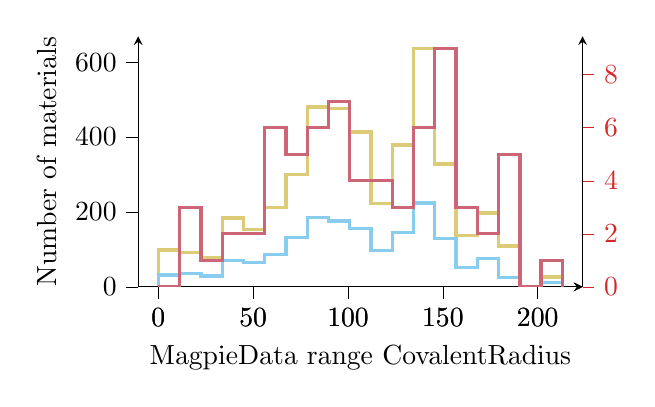
\begin{tikzpicture}

\definecolor{color0}{rgb}{0.866666666666667,0.8,0.466666666666667}
\definecolor{color1}{rgb}{0.533333333333333,0.8,0.933333333333333}
\definecolor{color2}{rgb}{0.83921568627451,0.152941176470588,0.156862745098039}
\definecolor{color3}{rgb}{0.8,0.4,0.466666666666667}

\begin{axis}[
height=1.875590092707901in,
legend cell align={left},
legend style={fill opacity=0.8, draw opacity=1, text opacity=1, draw=white!80!black},
tick align=outside,
tick pos=left,
width=2.8444876158848764in,
x grid style={white!69.0196078431373!black},
xlabel={MagpieData range CovalentRadius},
xmin=-10.65, xmax=223.65,
xtick style={color=black},
y grid style={white!69.0196078431373!black},
ylabel={Number of materials},
ymin=0, ymax=668.85,
ytick style={color=black}
]
\path [draw=color0, very thick]
(axis cs:0,0)
--(axis cs:0,98)
--(axis cs:11.2105263157895,98)
--(axis cs:11.2105263157895,92)
--(axis cs:22.4210526315789,92)
--(axis cs:22.4210526315789,79)
--(axis cs:33.6315789473684,79)
--(axis cs:33.6315789473684,184)
--(axis cs:44.8421052631579,184)
--(axis cs:44.8421052631579,154)
--(axis cs:56.0526315789474,154)
--(axis cs:56.0526315789474,211)
--(axis cs:67.2631578947368,211)
--(axis cs:67.2631578947368,300)
--(axis cs:78.4736842105263,300)
--(axis cs:78.4736842105263,480)
--(axis cs:89.6842105263158,480)
--(axis cs:89.6842105263158,477)
--(axis cs:100.894736842105,477)
--(axis cs:100.894736842105,413)
--(axis cs:112.105263157895,413)
--(axis cs:112.105263157895,223)
--(axis cs:123.315789473684,223)
--(axis cs:123.315789473684,379)
--(axis cs:134.526315789474,379)
--(axis cs:134.526315789474,637)
--(axis cs:145.736842105263,637)
--(axis cs:145.736842105263,328)
--(axis cs:156.947368421053,328)
--(axis cs:156.947368421053,138)
--(axis cs:168.157894736842,138)
--(axis cs:168.157894736842,197)
--(axis cs:179.368421052632,197)
--(axis cs:179.368421052632,109)
--(axis cs:190.578947368421,109)
--(axis cs:190.578947368421,0)
--(axis cs:201.789473684211,0)
--(axis cs:201.789473684211,26)
--(axis cs:213,26)
--(axis cs:213,0);

\path [draw=color1, very thick]
(axis cs:0,0)
--(axis cs:0,32)
--(axis cs:11.2105263157895,32)
--(axis cs:11.2105263157895,36)
--(axis cs:22.4210526315789,36)
--(axis cs:22.4210526315789,29)
--(axis cs:33.6315789473684,29)
--(axis cs:33.6315789473684,71)
--(axis cs:44.8421052631579,71)
--(axis cs:44.8421052631579,65)
--(axis cs:56.0526315789474,65)
--(axis cs:56.0526315789474,87)
--(axis cs:67.2631578947368,87)
--(axis cs:67.2631578947368,132)
--(axis cs:78.4736842105263,132)
--(axis cs:78.4736842105263,186)
--(axis cs:89.6842105263158,186)
--(axis cs:89.6842105263158,176)
--(axis cs:100.894736842105,176)
--(axis cs:100.894736842105,156)
--(axis cs:112.105263157895,156)
--(axis cs:112.105263157895,97)
--(axis cs:123.315789473684,97)
--(axis cs:123.315789473684,145)
--(axis cs:134.526315789474,145)
--(axis cs:134.526315789474,224)
--(axis cs:145.736842105263,224)
--(axis cs:145.736842105263,130)
--(axis cs:156.947368421053,130)
--(axis cs:156.947368421053,51)
--(axis cs:168.157894736842,51)
--(axis cs:168.157894736842,76)
--(axis cs:179.368421052632,76)
--(axis cs:179.368421052632,25)
--(axis cs:190.578947368421,25)
--(axis cs:190.578947368421,0)
--(axis cs:201.789473684211,0)
--(axis cs:201.789473684211,11)
--(axis cs:213,11)
--(axis cs:213,0);

\end{axis}

\begin{axis}[
axis y line=right,
height=1.875590092707901in,
tick align=outside,
width=2.8444876158848764in,
x grid style={white!69.0196078431373!black},
xmin=-10.65, xmax=223.65,
xtick pos=left,
xtick style={color=black},
y grid style={white!69.0196078431373!black},
ymin=0, ymax=9.45,
ytick pos=right,
ytick style={color=color2},
yticklabel style={anchor=west, color2}
]
\path [draw=color3, very thick]
(axis cs:0,0)
--(axis cs:0,0)
--(axis cs:11.2105263157895,0)
--(axis cs:11.2105263157895,3)
--(axis cs:22.4210526315789,3)
--(axis cs:22.4210526315789,1)
--(axis cs:33.6315789473684,1)
--(axis cs:33.6315789473684,2)
--(axis cs:44.8421052631579,2)
--(axis cs:44.8421052631579,2)
--(axis cs:56.0526315789474,2)
--(axis cs:56.0526315789474,6)
--(axis cs:67.2631578947368,6)
--(axis cs:67.2631578947368,5)
--(axis cs:78.4736842105263,5)
--(axis cs:78.4736842105263,6)
--(axis cs:89.6842105263158,6)
--(axis cs:89.6842105263158,7)
--(axis cs:100.894736842105,7)
--(axis cs:100.894736842105,4)
--(axis cs:112.105263157895,4)
--(axis cs:112.105263157895,4)
--(axis cs:123.315789473684,4)
--(axis cs:123.315789473684,3)
--(axis cs:134.526315789474,3)
--(axis cs:134.526315789474,6)
--(axis cs:145.736842105263,6)
--(axis cs:145.736842105263,9)
--(axis cs:156.947368421053,9)
--(axis cs:156.947368421053,3)
--(axis cs:168.157894736842,3)
--(axis cs:168.157894736842,2)
--(axis cs:179.368421052632,2)
--(axis cs:179.368421052632,5)
--(axis cs:190.578947368421,5)
--(axis cs:190.578947368421,0)
--(axis cs:201.789473684211,0)
--(axis cs:201.789473684211,1)
--(axis cs:213,1)
--(axis cs:213,0);
\end{axis}

\end{tikzpicture}
}
    \subcaption{}
\end{subfigure}
\begin{subfigure}[b]{0.45\textwidth}
    \scalebox{0.85}{% This file was created with tikzplotlib v0.9.16.
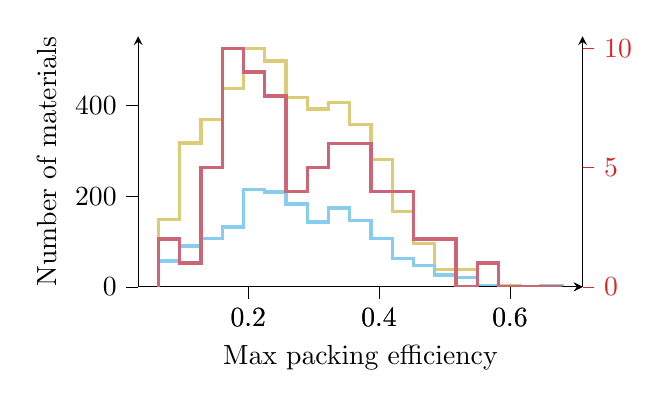
\begin{tikzpicture}

\definecolor{color0}{rgb}{0.866666666666667,0.8,0.466666666666667}
\definecolor{color1}{rgb}{0.533333333333333,0.8,0.933333333333333}
\definecolor{color2}{rgb}{0.83921568627451,0.152941176470588,0.156862745098039}
\definecolor{color3}{rgb}{0.8,0.4,0.466666666666667}

\begin{axis}[
height=1.875590092707901in,
legend cell align={left},
legend style={fill opacity=0.8, draw opacity=1, text opacity=1, draw=white!80!black},
tick align=outside,
tick pos=left,
width=2.8444876158848764in,
x grid style={white!69.0196078431373!black},
xlabel={Max packing efficiency},
xmin=0.0318178138255053, xmax=0.711048901957466,
xtick style={color=black},
y grid style={white!69.0196078431373!black},
ylabel={Number of materials},
ymin=0, ymax=552.3,
ytick style={color=black}
]
\path [draw=color0, very thick]
(axis cs:0.0626919541951399,0)
--(axis cs:0.0626919541951399,148)
--(axis cs:0.0951910493210711,148)
--(axis cs:0.0951910493210711,317)
--(axis cs:0.127690144447002,317)
--(axis cs:0.127690144447002,369)
--(axis cs:0.160189239572933,369)
--(axis cs:0.160189239572933,437)
--(axis cs:0.192688334698864,437)
--(axis cs:0.192688334698864,526)
--(axis cs:0.225187429824796,526)
--(axis cs:0.225187429824796,498)
--(axis cs:0.257686524950727,498)
--(axis cs:0.257686524950727,418)
--(axis cs:0.290185620076658,418)
--(axis cs:0.290185620076658,392)
--(axis cs:0.322684715202589,392)
--(axis cs:0.322684715202589,407)
--(axis cs:0.35518381032852,407)
--(axis cs:0.35518381032852,358)
--(axis cs:0.387682905454451,358)
--(axis cs:0.387682905454451,281)
--(axis cs:0.420182000580382,281)
--(axis cs:0.420182000580382,166)
--(axis cs:0.452681095706314,166)
--(axis cs:0.452681095706314,95)
--(axis cs:0.485180190832245,95)
--(axis cs:0.485180190832245,39)
--(axis cs:0.517679285958176,39)
--(axis cs:0.517679285958176,38)
--(axis cs:0.550178381084107,38)
--(axis cs:0.550178381084107,3)
--(axis cs:0.582677476210038,3)
--(axis cs:0.582677476210038,2)
--(axis cs:0.615176571335969,2)
--(axis cs:0.615176571335969,1)
--(axis cs:0.6476756664619,1)
--(axis cs:0.6476756664619,3)
--(axis cs:0.680174761587832,3)
--(axis cs:0.680174761587832,0);

\path [draw=color1, very thick]
(axis cs:0.0626919541951399,0)
--(axis cs:0.0626919541951399,57)
--(axis cs:0.0951910493210711,57)
--(axis cs:0.0951910493210711,90)
--(axis cs:0.127690144447002,90)
--(axis cs:0.127690144447002,107)
--(axis cs:0.160189239572933,107)
--(axis cs:0.160189239572933,132)
--(axis cs:0.192688334698864,132)
--(axis cs:0.192688334698864,215)
--(axis cs:0.225187429824796,215)
--(axis cs:0.225187429824796,209)
--(axis cs:0.257686524950727,209)
--(axis cs:0.257686524950727,183)
--(axis cs:0.290185620076658,183)
--(axis cs:0.290185620076658,143)
--(axis cs:0.322684715202589,143)
--(axis cs:0.322684715202589,174)
--(axis cs:0.35518381032852,174)
--(axis cs:0.35518381032852,146)
--(axis cs:0.387682905454451,146)
--(axis cs:0.387682905454451,106)
--(axis cs:0.420182000580382,106)
--(axis cs:0.420182000580382,63)
--(axis cs:0.452681095706314,63)
--(axis cs:0.452681095706314,47)
--(axis cs:0.485180190832245,47)
--(axis cs:0.485180190832245,26)
--(axis cs:0.517679285958176,26)
--(axis cs:0.517679285958176,21)
--(axis cs:0.550178381084107,21)
--(axis cs:0.550178381084107,3)
--(axis cs:0.582677476210038,3)
--(axis cs:0.582677476210038,0)
--(axis cs:0.615176571335969,0)
--(axis cs:0.615176571335969,0)
--(axis cs:0.6476756664619,0)
--(axis cs:0.6476756664619,3)
--(axis cs:0.680174761587832,3)
--(axis cs:0.680174761587832,0);

\end{axis}

\begin{axis}[
axis y line=right,
height=1.875590092707901in,
tick align=outside,
width=2.8444876158848764in,
x grid style={white!69.0196078431373!black},
xmin=0.0318178138255053, xmax=0.711048901957466,
xtick pos=left,
xtick style={color=black},
y grid style={white!69.0196078431373!black},
ymin=0, ymax=10.5,
ytick pos=right,
ytick style={color=color2},
yticklabel style={anchor=west, color=color2}
]
\path [draw=color3, very thick]
(axis cs:0.0626919541951399,0)
--(axis cs:0.0626919541951399,2)
--(axis cs:0.0951910493210711,2)
--(axis cs:0.0951910493210711,1)
--(axis cs:0.127690144447002,1)
--(axis cs:0.127690144447002,5)
--(axis cs:0.160189239572933,5)
--(axis cs:0.160189239572933,10)
--(axis cs:0.192688334698864,10)
--(axis cs:0.192688334698864,9)
--(axis cs:0.225187429824796,9)
--(axis cs:0.225187429824796,8)
--(axis cs:0.257686524950727,8)
--(axis cs:0.257686524950727,4)
--(axis cs:0.290185620076658,4)
--(axis cs:0.290185620076658,5)
--(axis cs:0.322684715202589,5)
--(axis cs:0.322684715202589,6)
--(axis cs:0.35518381032852,6)
--(axis cs:0.35518381032852,6)
--(axis cs:0.387682905454451,6)
--(axis cs:0.387682905454451,4)
--(axis cs:0.420182000580382,4)
--(axis cs:0.420182000580382,4)
--(axis cs:0.452681095706314,4)
--(axis cs:0.452681095706314,2)
--(axis cs:0.485180190832245,2)
--(axis cs:0.485180190832245,2)
--(axis cs:0.517679285958176,2)
--(axis cs:0.517679285958176,0)
--(axis cs:0.550178381084107,0)
--(axis cs:0.550178381084107,1)
--(axis cs:0.582677476210038,1)
--(axis cs:0.582677476210038,0)
--(axis cs:0.615176571335969,0)
--(axis cs:0.615176571335969,0)
--(axis cs:0.6476756664619,0)
--(axis cs:0.6476756664619,0)
--(axis cs:0.680174761587832,0)
--(axis cs:0.680174761587832,0);
\end{axis}

\end{tikzpicture}
}
    \subcaption{}
\end{subfigure}%

\begin{subfigure}[b]{0.45\textwidth}
    \scalebox{0.85}{% This file was created with tikzplotlib v0.9.16.
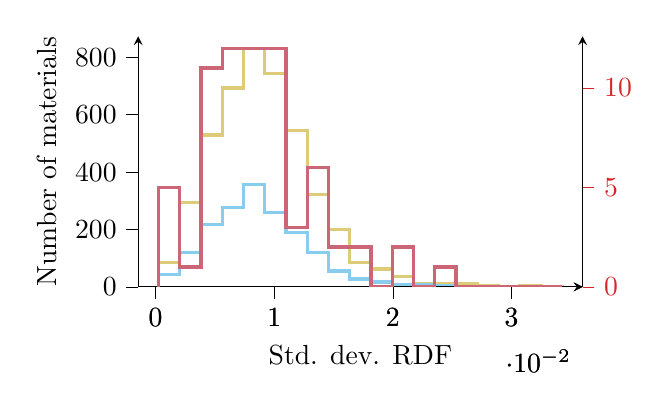
\begin{tikzpicture}

\definecolor{color0}{rgb}{0.866666666666667,0.8,0.466666666666667}
\definecolor{color1}{rgb}{0.533333333333333,0.8,0.933333333333333}
\definecolor{color2}{rgb}{0.83921568627451,0.152941176470588,0.156862745098039}
\definecolor{color3}{rgb}{0.8,0.4,0.466666666666667}

\begin{axis}[
height=1.875590092707901in,
legend cell align={left},
legend style={fill opacity=0.8, draw opacity=1, text opacity=1, draw=white!80!black},
tick align=outside,
tick pos=left,
width=2.8444876158848764in,
x grid style={white!69.0196078431373!black},
xlabel={Std. dev. RDF},
xmin=-0.00146657305751061, xmax=0.0359919745342756,
xtick style={color=black},
y grid style={white!69.0196078431373!black},
ylabel={Number of materials},
ymin=0, ymax=873.6,
ytick style={color=black}
]
\path [draw=color0, very thick]
(axis cs:0.000236088196661485,0)
--(axis cs:0.000236088196661485,84)
--(axis cs:0.00202836320105317,84)
--(axis cs:0.00202836320105317,293)
--(axis cs:0.00382063820544485,293)
--(axis cs:0.00382063820544485,530)
--(axis cs:0.00561291320983653,530)
--(axis cs:0.00561291320983653,693)
--(axis cs:0.00740518821422822,693)
--(axis cs:0.00740518821422822,832)
--(axis cs:0.0091974632186199,832)
--(axis cs:0.0091974632186199,743)
--(axis cs:0.0109897382230116,743)
--(axis cs:0.0109897382230116,544)
--(axis cs:0.0127820132274033,544)
--(axis cs:0.0127820132274033,322)
--(axis cs:0.0145742882317949,322)
--(axis cs:0.0145742882317949,200)
--(axis cs:0.0163665632361866,200)
--(axis cs:0.0163665632361866,85)
--(axis cs:0.0181588382405783,85)
--(axis cs:0.0181588382405783,62)
--(axis cs:0.01995111324497,62)
--(axis cs:0.01995111324497,37)
--(axis cs:0.0217433882493617,37)
--(axis cs:0.0217433882493617,11)
--(axis cs:0.0235356632537534,11)
--(axis cs:0.0235356632537534,12)
--(axis cs:0.025327938258145,12)
--(axis cs:0.025327938258145,10)
--(axis cs:0.0271202132625367,10)
--(axis cs:0.0271202132625367,5)
--(axis cs:0.0289124882669284,5)
--(axis cs:0.0289124882669284,0)
--(axis cs:0.0307047632713201,0)
--(axis cs:0.0307047632713201,3)
--(axis cs:0.0324970382757118,3)
--(axis cs:0.0324970382757118,1)
--(axis cs:0.0342893132801035,1)
--(axis cs:0.0342893132801035,0);

\path [draw=color1, very thick]
(axis cs:0.000236088196661485,0)
--(axis cs:0.000236088196661485,42)
--(axis cs:0.00202836320105317,42)
--(axis cs:0.00202836320105317,119)
--(axis cs:0.00382063820544485,119)
--(axis cs:0.00382063820544485,217)
--(axis cs:0.00561291320983653,217)
--(axis cs:0.00561291320983653,276)
--(axis cs:0.00740518821422822,276)
--(axis cs:0.00740518821422822,356)
--(axis cs:0.0091974632186199,356)
--(axis cs:0.0091974632186199,260)
--(axis cs:0.0109897382230116,260)
--(axis cs:0.0109897382230116,190)
--(axis cs:0.0127820132274033,190)
--(axis cs:0.0127820132274033,119)
--(axis cs:0.0145742882317949,119)
--(axis cs:0.0145742882317949,55)
--(axis cs:0.0163665632361866,55)
--(axis cs:0.0163665632361866,28)
--(axis cs:0.0181588382405783,28)
--(axis cs:0.0181588382405783,17)
--(axis cs:0.01995111324497,17)
--(axis cs:0.01995111324497,7)
--(axis cs:0.0217433882493617,7)
--(axis cs:0.0217433882493617,8)
--(axis cs:0.0235356632537534,8)
--(axis cs:0.0235356632537534,4)
--(axis cs:0.025327938258145,4)
--(axis cs:0.025327938258145,0)
--(axis cs:0.0271202132625367,0)
--(axis cs:0.0271202132625367,2)
--(axis cs:0.0289124882669284,2)
--(axis cs:0.0289124882669284,1)
--(axis cs:0.0307047632713201,1)
--(axis cs:0.0307047632713201,1)
--(axis cs:0.0324970382757118,1)
--(axis cs:0.0324970382757118,0)
--(axis cs:0.0342893132801035,0)
--(axis cs:0.0342893132801035,0);

\end{axis}

\begin{axis}[
axis y line=right,
height=1.875590092707901in,
tick align=outside,
width=2.8444876158848764in,
x grid style={white!69.0196078431373!black},
xmin=-0.00146657305751061, xmax=0.0359919745342756,
xtick pos=left,
xtick style={color=black},
y grid style={white!69.0196078431373!black},
ymin=0, ymax=12.6,
ytick pos=right,
ytick style={color=color2},
yticklabel style={anchor=west, color=color2}
]
\path [draw=color3, very thick]
(axis cs:0.000236088196661485,0)
--(axis cs:0.000236088196661485,5)
--(axis cs:0.00202836320105317,5)
--(axis cs:0.00202836320105317,1)
--(axis cs:0.00382063820544485,1)
--(axis cs:0.00382063820544485,11)
--(axis cs:0.00561291320983653,11)
--(axis cs:0.00561291320983653,12)
--(axis cs:0.00740518821422822,12)
--(axis cs:0.00740518821422822,12)
--(axis cs:0.0091974632186199,12)
--(axis cs:0.0091974632186199,12)
--(axis cs:0.0109897382230116,12)
--(axis cs:0.0109897382230116,3)
--(axis cs:0.0127820132274033,3)
--(axis cs:0.0127820132274033,6)
--(axis cs:0.0145742882317949,6)
--(axis cs:0.0145742882317949,2)
--(axis cs:0.0163665632361866,2)
--(axis cs:0.0163665632361866,2)
--(axis cs:0.0181588382405783,2)
--(axis cs:0.0181588382405783,0)
--(axis cs:0.01995111324497,0)
--(axis cs:0.01995111324497,2)
--(axis cs:0.0217433882493617,2)
--(axis cs:0.0217433882493617,0)
--(axis cs:0.0235356632537534,0)
--(axis cs:0.0235356632537534,1)
--(axis cs:0.025327938258145,1)
--(axis cs:0.025327938258145,0)
--(axis cs:0.0271202132625367,0)
--(axis cs:0.0271202132625367,0)
--(axis cs:0.0289124882669284,0)
--(axis cs:0.0289124882669284,0)
--(axis cs:0.0307047632713201,0)
--(axis cs:0.0307047632713201,0)
--(axis cs:0.0324970382757118,0)
--(axis cs:0.0324970382757118,0)
--(axis cs:0.0342893132801035,0)
--(axis cs:0.0342893132801035,0);
\end{axis}

\end{tikzpicture}
}
    \subcaption{}
\end{subfigure}
\begin{subfigure}[b]{0.45\textwidth}
    \scalebox{0.85}{% This file was created with tikzplotlib v0.9.16.
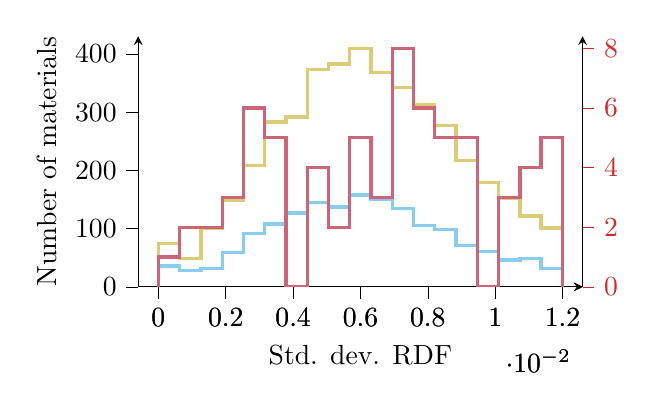
\begin{tikzpicture}

\definecolor{color0}{rgb}{0.866666666666667,0.8,0.466666666666667}
\definecolor{color1}{rgb}{0.533333333333333,0.8,0.933333333333333}
\definecolor{color2}{rgb}{0.83921568627451,0.152941176470588,0.156862745098039}
\definecolor{color3}{rgb}{0.8,0.4,0.466666666666667}

\begin{axis}[
height=1.875590092707901in,
legend cell align={left},
legend style={fill opacity=0.8, draw opacity=1, text opacity=1, draw=white!80!black},
tick align=outside,
tick pos=left,
width=2.8444876158848764in,
x grid style={white!69.0196078431373!black},
xlabel={Std. dev. RDF},
xmin=-0.000599766697946528, xmax=0.0125951006568771,
xtick style={color=black},
y grid style={white!69.0196078431373!black},
ylabel={Number of materials},
ymin=0, ymax=430.5,
ytick style={color=black}
]
\path [draw=color0, very thick]
(axis cs:0,0)
--(axis cs:0,74)
--(axis cs:0.000631333366259504,74)
--(axis cs:0.000631333366259504,49)
--(axis cs:0.00126266673251901,49)
--(axis cs:0.00126266673251901,100)
--(axis cs:0.00189400009877851,100)
--(axis cs:0.00189400009877851,148)
--(axis cs:0.00252533346503801,148)
--(axis cs:0.00252533346503801,208)
--(axis cs:0.00315666683129752,208)
--(axis cs:0.00315666683129752,283)
--(axis cs:0.00378800019755702,283)
--(axis cs:0.00378800019755702,292)
--(axis cs:0.00441933356381652,292)
--(axis cs:0.00441933356381652,373)
--(axis cs:0.00505066693007603,373)
--(axis cs:0.00505066693007603,383)
--(axis cs:0.00568200029633553,383)
--(axis cs:0.00568200029633553,410)
--(axis cs:0.00631333366259504,410)
--(axis cs:0.00631333366259504,368)
--(axis cs:0.00694466702885454,368)
--(axis cs:0.00694466702885454,343)
--(axis cs:0.00757600039511404,343)
--(axis cs:0.00757600039511404,313)
--(axis cs:0.00820733376137354,313)
--(axis cs:0.00820733376137354,277)
--(axis cs:0.00883866712763305,277)
--(axis cs:0.00883866712763305,217)
--(axis cs:0.00947000049389255,217)
--(axis cs:0.00947000049389255,179)
--(axis cs:0.0101013338601521,179)
--(axis cs:0.0101013338601521,152)
--(axis cs:0.0107326672264116,152)
--(axis cs:0.0107326672264116,122)
--(axis cs:0.0113640005926711,122)
--(axis cs:0.0113640005926711,101)
--(axis cs:0.0119953339589306,101)
--(axis cs:0.0119953339589306,0);

\path [draw=color1, very thick]
(axis cs:0,0)
--(axis cs:0,36)
--(axis cs:0.000631333366259504,36)
--(axis cs:0.000631333366259504,28)
--(axis cs:0.00126266673251901,28)
--(axis cs:0.00126266673251901,31)
--(axis cs:0.00189400009877851,31)
--(axis cs:0.00189400009877851,59)
--(axis cs:0.00252533346503801,59)
--(axis cs:0.00252533346503801,92)
--(axis cs:0.00315666683129752,92)
--(axis cs:0.00315666683129752,108)
--(axis cs:0.00378800019755702,108)
--(axis cs:0.00378800019755702,127)
--(axis cs:0.00441933356381652,127)
--(axis cs:0.00441933356381652,145)
--(axis cs:0.00505066693007603,145)
--(axis cs:0.00505066693007603,137)
--(axis cs:0.00568200029633553,137)
--(axis cs:0.00568200029633553,158)
--(axis cs:0.00631333366259504,158)
--(axis cs:0.00631333366259504,151)
--(axis cs:0.00694466702885454,151)
--(axis cs:0.00694466702885454,135)
--(axis cs:0.00757600039511404,135)
--(axis cs:0.00757600039511404,106)
--(axis cs:0.00820733376137354,106)
--(axis cs:0.00820733376137354,98)
--(axis cs:0.00883866712763305,98)
--(axis cs:0.00883866712763305,71)
--(axis cs:0.00947000049389255,71)
--(axis cs:0.00947000049389255,61)
--(axis cs:0.0101013338601521,61)
--(axis cs:0.0101013338601521,46)
--(axis cs:0.0107326672264116,46)
--(axis cs:0.0107326672264116,49)
--(axis cs:0.0113640005926711,49)
--(axis cs:0.0113640005926711,31)
--(axis cs:0.0119953339589306,31)
--(axis cs:0.0119953339589306,0);

\end{axis}

\begin{axis}[
axis y line=right,
height=1.875590092707901in,
tick align=outside,
width=2.8444876158848764in,
x grid style={white!69.0196078431373!black},
xmin=-0.000599766697946528, xmax=0.0125951006568771,
xtick pos=left,
xtick style={color=black},
y grid style={white!69.0196078431373!black},
ymin=0, ymax=8.4,
ytick pos=right,
ytick style={color=color2},
yticklabel style={anchor=west, color=color2}
]
\path [draw=color3, very thick]
(axis cs:0,0)
--(axis cs:0,1)
--(axis cs:0.000631333366259504,1)
--(axis cs:0.000631333366259504,2)
--(axis cs:0.00126266673251901,2)
--(axis cs:0.00126266673251901,2)
--(axis cs:0.00189400009877851,2)
--(axis cs:0.00189400009877851,3)
--(axis cs:0.00252533346503801,3)
--(axis cs:0.00252533346503801,6)
--(axis cs:0.00315666683129752,6)
--(axis cs:0.00315666683129752,5)
--(axis cs:0.00378800019755702,5)
--(axis cs:0.00378800019755702,0)
--(axis cs:0.00441933356381652,0)
--(axis cs:0.00441933356381652,4)
--(axis cs:0.00505066693007603,4)
--(axis cs:0.00505066693007603,2)
--(axis cs:0.00568200029633553,2)
--(axis cs:0.00568200029633553,5)
--(axis cs:0.00631333366259504,5)
--(axis cs:0.00631333366259504,3)
--(axis cs:0.00694466702885454,3)
--(axis cs:0.00694466702885454,8)
--(axis cs:0.00757600039511404,8)
--(axis cs:0.00757600039511404,6)
--(axis cs:0.00820733376137354,6)
--(axis cs:0.00820733376137354,5)
--(axis cs:0.00883866712763305,5)
--(axis cs:0.00883866712763305,5)
--(axis cs:0.00947000049389255,5)
--(axis cs:0.00947000049389255,0)
--(axis cs:0.0101013338601521,0)
--(axis cs:0.0101013338601521,3)
--(axis cs:0.0107326672264116,3)
--(axis cs:0.0107326672264116,4)
--(axis cs:0.0113640005926711,4)
--(axis cs:0.0113640005926711,5)
--(axis cs:0.0119953339589306,5)
--(axis cs:0.0119953339589306,0);
\end{axis}

\end{tikzpicture}
}
    \subcaption{}
\end{subfigure}%
\caption{Number of predicted suitable materials as a function of the (a) covalent radius, (b) maximum packing efficiency, and standard deviation of the radial distribution function with center at (c) $2.0$ and (d) $3.0$. 
The Ferrenti and extended Ferrenti approaches refer to the left y-axis and the empirical approach to the right. All panels were taken for a $0.75$ cut-off. }
\label{fig:histograms_supp1}
\end{figure}

Figure~\ref{fig:histograms_supp1} displays the number of predicted suitable materials for all approaches (all ML methods in an approach agree to a $0.75$ confidence level) as a function of the (a) covalent radius of the elements in the composition, (b) maximum packing efficiency, and standard deviation of the radial distribution function (RDF) with center at (c) $2.0$ and (d) $3.0$. The corresponding figure in the main text shows the standard deviation of the RDF with Gaussian center at $1.0$. 

We observe that the covalent radii of the materials (see Fig.~\ref{fig:histograms_supp1}a) distribute with two peaks in the data in all approaches. The maxima are slightly shifted towards the right for the empirical approach compared to the two others but otherwise the data distributions are similar. The trend of two data peaks is repeated for the maximum packing efficiency (see Fig.~\ref{fig:histograms_supp1}b) but is much more prominent for the empirical approach. This indicates that the material density, or in other words the bond length, is an important parameter for QT suitability.  

\begin{figure}[ht!]
\begin{subfigure}[t]{1\textwidth}
    % This file was created by tikzplotlib v0.9.8.
\begin{tikzpicture}

\definecolor{color0}{rgb}{0.866666666666667,0.8,0.466666666666667}
\definecolor{color1}{rgb}{0.533333333333333,0.8,0.933333333333333}
\definecolor{color3}{rgb}{0.8,0.4,0.466666666666667}
\begin{axis}[%
 hide axis,
 xmin=10,
 xmax=11,
 ymin=0,
 ymax=0.4,
 legend columns=,
 legend style={
   fill opacity=1,
   draw opacity=1,
   text opacity=1,
   align=center,
   anchor=north,
   draw=white!80!black
 },
 ]
 \addlegendimage{semithick, color1}
 \addlegendentry{Ferrenti approach};
 \addlegendimage{semithick, color0}
 \addlegendentry{Extended Ferrenti approach};
 \addlegendimage{semithick, color3}
 \addlegendentry{Empirical approach};
 \end{axis}

\end{tikzpicture}

\end{subfigure}
\begin{subfigure}[b]{0.45\textwidth}
    \scalebox{0.85}{% This file was created with tikzplotlib v0.9.16.
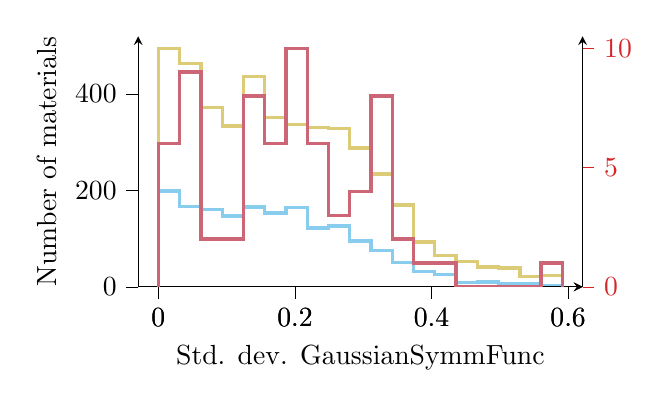
\begin{tikzpicture}

\definecolor{color0}{rgb}{0.866666666666667,0.8,0.466666666666667}
\definecolor{color1}{rgb}{0.533333333333333,0.8,0.933333333333333}
\definecolor{color2}{rgb}{0.83921568627451,0.152941176470588,0.156862745098039}
\definecolor{color3}{rgb}{0.8,0.4,0.466666666666667}

\begin{axis}[
height=1.875590092707901in,
legend cell align={left},
legend style={fill opacity=0.8, draw opacity=1, text opacity=1, draw=white!80!black},
tick align=outside,
tick pos=left,
width=2.8444876158848764in,
x grid style={white!69.0196078431373!black},
xlabel={Std. dev. GaussianSymmFunc},
xmin=-0.0295818294063694, xmax=0.621218417533758,
xtick style={color=black},
y grid style={white!69.0196078431373!black},
ylabel={Number of materials},
ymin=0, ymax=519.75,
ytick style={color=black}
]
\path [draw=color0, very thick]
(axis cs:0,0)
--(axis cs:0,495)
--(axis cs:0.0311387677961784,495)
--(axis cs:0.0311387677961784,464)
--(axis cs:0.0622775355923567,464)
--(axis cs:0.0622775355923567,372)
--(axis cs:0.0934163033885351,372)
--(axis cs:0.0934163033885351,334)
--(axis cs:0.124555071184713,334)
--(axis cs:0.124555071184713,437)
--(axis cs:0.155693838980892,437)
--(axis cs:0.155693838980892,351)
--(axis cs:0.18683260677707,351)
--(axis cs:0.18683260677707,337)
--(axis cs:0.217971374573249,337)
--(axis cs:0.217971374573249,331)
--(axis cs:0.249110142369427,331)
--(axis cs:0.249110142369427,329)
--(axis cs:0.280248910165605,329)
--(axis cs:0.280248910165605,288)
--(axis cs:0.311387677961784,288)
--(axis cs:0.311387677961784,234)
--(axis cs:0.342526445757962,234)
--(axis cs:0.342526445757962,170)
--(axis cs:0.37366521355414,170)
--(axis cs:0.37366521355414,93)
--(axis cs:0.404803981350319,93)
--(axis cs:0.404803981350319,65)
--(axis cs:0.435942749146497,65)
--(axis cs:0.435942749146497,52)
--(axis cs:0.467081516942676,52)
--(axis cs:0.467081516942676,41)
--(axis cs:0.498220284738854,41)
--(axis cs:0.498220284738854,39)
--(axis cs:0.529359052535032,39)
--(axis cs:0.529359052535032,22)
--(axis cs:0.560497820331211,22)
--(axis cs:0.560497820331211,23)
--(axis cs:0.591636588127389,23)
--(axis cs:0.591636588127389,0);

\path [draw=color1, very thick]
(axis cs:0,0)
--(axis cs:0,199)
--(axis cs:0.0311387677961784,199)
--(axis cs:0.0311387677961784,167)
--(axis cs:0.0622775355923567,167)
--(axis cs:0.0622775355923567,160)
--(axis cs:0.0934163033885351,160)
--(axis cs:0.0934163033885351,147)
--(axis cs:0.124555071184713,147)
--(axis cs:0.124555071184713,166)
--(axis cs:0.155693838980892,166)
--(axis cs:0.155693838980892,153)
--(axis cs:0.18683260677707,153)
--(axis cs:0.18683260677707,164)
--(axis cs:0.217971374573249,164)
--(axis cs:0.217971374573249,122)
--(axis cs:0.249110142369427,122)
--(axis cs:0.249110142369427,126)
--(axis cs:0.280248910165605,126)
--(axis cs:0.280248910165605,95)
--(axis cs:0.311387677961784,95)
--(axis cs:0.311387677961784,75)
--(axis cs:0.342526445757962,75)
--(axis cs:0.342526445757962,50)
--(axis cs:0.37366521355414,50)
--(axis cs:0.37366521355414,32)
--(axis cs:0.404803981350319,32)
--(axis cs:0.404803981350319,26)
--(axis cs:0.435942749146497,26)
--(axis cs:0.435942749146497,9)
--(axis cs:0.467081516942676,9)
--(axis cs:0.467081516942676,10)
--(axis cs:0.498220284738854,10)
--(axis cs:0.498220284738854,7)
--(axis cs:0.529359052535032,7)
--(axis cs:0.529359052535032,7)
--(axis cs:0.560497820331211,7)
--(axis cs:0.560497820331211,3)
--(axis cs:0.591636588127389,3)
--(axis cs:0.591636588127389,0);

\end{axis}

\begin{axis}[
axis y line=right,
height=1.875590092707901in,
tick align=outside,
width=2.8444876158848764in,
x grid style={white!69.0196078431373!black},
xmin=-0.0295818294063694, xmax=0.621218417533758,
xtick pos=left,
xtick style={color=black},
y grid style={white!69.0196078431373!black},
ymin=0, ymax=10.5,
ytick pos=right,
ytick style={color=color2},
yticklabel style={anchor=west, color=color2}
]
\path [draw=color3, very thick]
(axis cs:0,0)
--(axis cs:0,6)
--(axis cs:0.0311387677961784,6)
--(axis cs:0.0311387677961784,9)
--(axis cs:0.0622775355923567,9)
--(axis cs:0.0622775355923567,2)
--(axis cs:0.0934163033885351,2)
--(axis cs:0.0934163033885351,2)
--(axis cs:0.124555071184713,2)
--(axis cs:0.124555071184713,8)
--(axis cs:0.155693838980892,8)
--(axis cs:0.155693838980892,6)
--(axis cs:0.18683260677707,6)
--(axis cs:0.18683260677707,10)
--(axis cs:0.217971374573249,10)
--(axis cs:0.217971374573249,6)
--(axis cs:0.249110142369427,6)
--(axis cs:0.249110142369427,3)
--(axis cs:0.280248910165605,3)
--(axis cs:0.280248910165605,4)
--(axis cs:0.311387677961784,4)
--(axis cs:0.311387677961784,8)
--(axis cs:0.342526445757962,8)
--(axis cs:0.342526445757962,2)
--(axis cs:0.37366521355414,2)
--(axis cs:0.37366521355414,1)
--(axis cs:0.404803981350319,1)
--(axis cs:0.404803981350319,1)
--(axis cs:0.435942749146497,1)
--(axis cs:0.435942749146497,0)
--(axis cs:0.467081516942676,0)
--(axis cs:0.467081516942676,0)
--(axis cs:0.498220284738854,0)
--(axis cs:0.498220284738854,0)
--(axis cs:0.529359052535032,0)
--(axis cs:0.529359052535032,0)
--(axis cs:0.560497820331211,0)
--(axis cs:0.560497820331211,1)
--(axis cs:0.591636588127389,1)
--(axis cs:0.591636588127389,0);
\end{axis}

\end{tikzpicture}
}
    \subcaption{}
\end{subfigure}
\begin{subfigure}[b]{0.45\textwidth}
    \scalebox{0.85}{% This file was created with tikzplotlib v0.9.16.
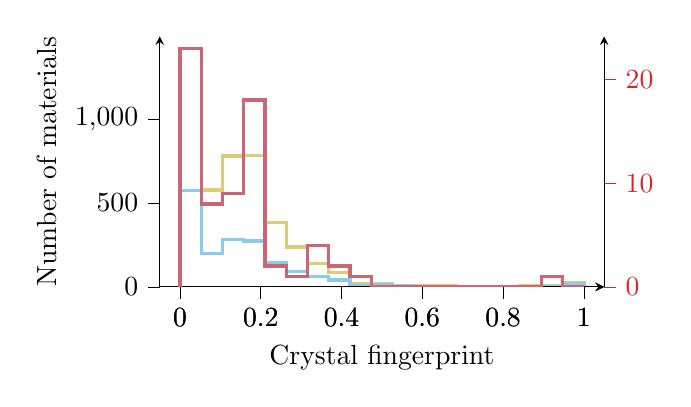
\begin{tikzpicture}

\definecolor{color0}{rgb}{0.866666666666667,0.8,0.466666666666667}
\definecolor{color1}{rgb}{0.533333333333333,0.8,0.933333333333333}
\definecolor{color2}{rgb}{0.83921568627451,0.152941176470588,0.156862745098039}
\definecolor{color3}{rgb}{0.8,0.4,0.466666666666667}

\begin{axis}[
height=1.875590092707901in,
legend cell align={left},
legend style={fill opacity=0.8, draw opacity=1, text opacity=1, draw=white!80!black},
tick align=outside,
tick pos=left,
width=2.8444876158848764in,
x grid style={white!69.0196078431373!black},
xlabel={Crystal fingerprint},
xmin=-0.05, xmax=1.05,
xtick style={color=black},
y grid style={white!69.0196078431373!black},
ylabel={Number of materials},
ymin=0, ymax=1492.05,
ytick style={color=black}
]
\path [draw=color0, very thick]
(axis cs:0,0)
--(axis cs:0,1421)
--(axis cs:0.0526315789473684,1421)
--(axis cs:0.0526315789473684,577)
--(axis cs:0.105263157894737,577)
--(axis cs:0.105263157894737,780)
--(axis cs:0.157894736842105,780)
--(axis cs:0.157894736842105,781)
--(axis cs:0.210526315789474,781)
--(axis cs:0.210526315789474,382)
--(axis cs:0.263157894736842,382)
--(axis cs:0.263157894736842,237)
--(axis cs:0.315789473684211,237)
--(axis cs:0.315789473684211,138)
--(axis cs:0.368421052631579,138)
--(axis cs:0.368421052631579,86)
--(axis cs:0.421052631578947,86)
--(axis cs:0.421052631578947,22)
--(axis cs:0.473684210526316,22)
--(axis cs:0.473684210526316,18)
--(axis cs:0.526315789473684,18)
--(axis cs:0.526315789473684,5)
--(axis cs:0.578947368421053,5)
--(axis cs:0.578947368421053,5)
--(axis cs:0.631578947368421,5)
--(axis cs:0.631578947368421,7)
--(axis cs:0.684210526315789,7)
--(axis cs:0.684210526315789,1)
--(axis cs:0.736842105263158,1)
--(axis cs:0.736842105263158,0)
--(axis cs:0.789473684210526,0)
--(axis cs:0.789473684210526,3)
--(axis cs:0.842105263157895,3)
--(axis cs:0.842105263157895,7)
--(axis cs:0.894736842105263,7)
--(axis cs:0.894736842105263,5)
--(axis cs:0.947368421052632,5)
--(axis cs:0.947368421052632,26)
--(axis cs:1,26)
--(axis cs:1,0);

\path [draw=color1, very thick]
(axis cs:0,0)
--(axis cs:0,574)
--(axis cs:0.0526315789473684,574)
--(axis cs:0.0526315789473684,197)
--(axis cs:0.105263157894737,197)
--(axis cs:0.105263157894737,283)
--(axis cs:0.157894736842105,283)
--(axis cs:0.157894736842105,274)
--(axis cs:0.210526315789474,274)
--(axis cs:0.210526315789474,146)
--(axis cs:0.263157894736842,146)
--(axis cs:0.263157894736842,91)
--(axis cs:0.315789473684211,91)
--(axis cs:0.315789473684211,63)
--(axis cs:0.368421052631579,63)
--(axis cs:0.368421052631579,40)
--(axis cs:0.421052631578947,40)
--(axis cs:0.421052631578947,7)
--(axis cs:0.473684210526316,7)
--(axis cs:0.473684210526316,11)
--(axis cs:0.526315789473684,11)
--(axis cs:0.526315789473684,5)
--(axis cs:0.578947368421053,5)
--(axis cs:0.578947368421053,2)
--(axis cs:0.631578947368421,2)
--(axis cs:0.631578947368421,4)
--(axis cs:0.684210526315789,4)
--(axis cs:0.684210526315789,0)
--(axis cs:0.736842105263158,0)
--(axis cs:0.736842105263158,2)
--(axis cs:0.789473684210526,2)
--(axis cs:0.789473684210526,2)
--(axis cs:0.842105263157895,2)
--(axis cs:0.842105263157895,1)
--(axis cs:0.894736842105263,1)
--(axis cs:0.894736842105263,3)
--(axis cs:0.947368421052632,3)
--(axis cs:0.947368421052632,19)
--(axis cs:1,19)
--(axis cs:1,0);

\end{axis}

\begin{axis}[
axis y line=right,
height=1.875590092707901in,
tick align=outside,
width=2.8444876158848764in,
x grid style={white!69.0196078431373!black},
xmin=-0.05, xmax=1.05,
xtick pos=left,
xtick style={color=black},
y grid style={white!69.0196078431373!black},
ymin=0, ymax=24.15,
ytick pos=right,
ytick style={color=color2},
yticklabel style={anchor=west,color=color2}
]
\path [draw=color3, very thick]
(axis cs:0,0)
--(axis cs:0,23)
--(axis cs:0.0526315789473684,23)
--(axis cs:0.0526315789473684,8)
--(axis cs:0.105263157894737,8)
--(axis cs:0.105263157894737,9)
--(axis cs:0.157894736842105,9)
--(axis cs:0.157894736842105,18)
--(axis cs:0.210526315789474,18)
--(axis cs:0.210526315789474,2)
--(axis cs:0.263157894736842,2)
--(axis cs:0.263157894736842,1)
--(axis cs:0.315789473684211,1)
--(axis cs:0.315789473684211,4)
--(axis cs:0.368421052631579,4)
--(axis cs:0.368421052631579,2)
--(axis cs:0.421052631578947,2)
--(axis cs:0.421052631578947,1)
--(axis cs:0.473684210526316,1)
--(axis cs:0.473684210526316,0)
--(axis cs:0.526315789473684,0)
--(axis cs:0.526315789473684,0)
--(axis cs:0.578947368421053,0)
--(axis cs:0.578947368421053,0)
--(axis cs:0.631578947368421,0)
--(axis cs:0.631578947368421,0)
--(axis cs:0.684210526315789,0)
--(axis cs:0.684210526315789,0)
--(axis cs:0.736842105263158,0)
--(axis cs:0.736842105263158,0)
--(axis cs:0.789473684210526,0)
--(axis cs:0.789473684210526,0)
--(axis cs:0.842105263157895,0)
--(axis cs:0.842105263157895,0)
--(axis cs:0.894736842105263,0)
--(axis cs:0.894736842105263,1)
--(axis cs:0.947368421052632,1)
--(axis cs:0.947368421052632,0)
--(axis cs:1,0)
--(axis cs:1,0);
\end{axis}

\end{tikzpicture}
}
    \subcaption{}
\end{subfigure}%

\begin{subfigure}[b]{0.45\textwidth}
    \scalebox{0.85}{% This file was created with tikzplotlib v0.9.16.
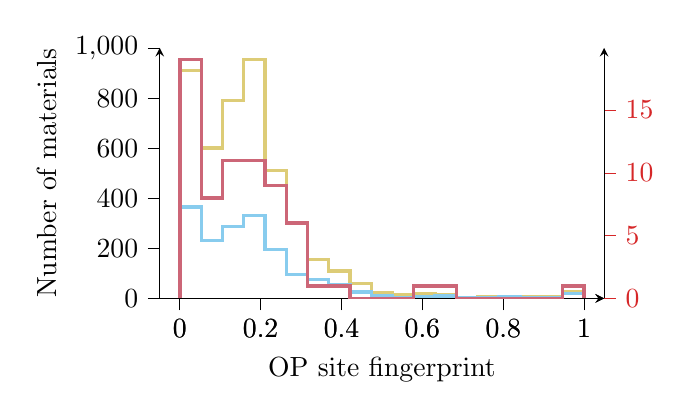
\begin{tikzpicture}

\definecolor{color0}{rgb}{0.866666666666667,0.8,0.466666666666667}
\definecolor{color1}{rgb}{0.533333333333333,0.8,0.933333333333333}
\definecolor{color2}{rgb}{0.83921568627451,0.152941176470588,0.156862745098039}
\definecolor{color3}{rgb}{0.8,0.4,0.466666666666667}

\begin{axis}[
height=1.875590092707901in,
legend cell align={left},
legend style={fill opacity=0.8, draw opacity=1, text opacity=1, draw=white!80!black},
tick align=outside,
tick pos=left,
width=2.8444876158848764in,
x grid style={white!69.0196078431373!black},
xlabel={OP site fingerprint},
xmin=-0.04945, xmax=1.04945,
xtick style={color=black},
y grid style={white!69.0196078431373!black},
ylabel={Number of materials},
ymin=0, ymax=1002.75,
ytick style={color=black}
]
\path [draw=color0, very thick]
(axis cs:0.0005,0)
--(axis cs:0.0005,913)
--(axis cs:0.0530789473684211,913)
--(axis cs:0.0530789473684211,602)
--(axis cs:0.105657894736842,602)
--(axis cs:0.105657894736842,793)
--(axis cs:0.158236842105263,793)
--(axis cs:0.158236842105263,955)
--(axis cs:0.210815789473684,955)
--(axis cs:0.210815789473684,512)
--(axis cs:0.263394736842105,512)
--(axis cs:0.263394736842105,301)
--(axis cs:0.315973684210526,301)
--(axis cs:0.315973684210526,156)
--(axis cs:0.368552631578947,156)
--(axis cs:0.368552631578947,110)
--(axis cs:0.421131578947369,110)
--(axis cs:0.421131578947369,61)
--(axis cs:0.47371052631579,61)
--(axis cs:0.47371052631579,24)
--(axis cs:0.526289473684211,24)
--(axis cs:0.526289473684211,16)
--(axis cs:0.578868421052632,16)
--(axis cs:0.578868421052632,17)
--(axis cs:0.631447368421053,17)
--(axis cs:0.631447368421053,15)
--(axis cs:0.684026315789474,15)
--(axis cs:0.684026315789474,4)
--(axis cs:0.736605263157895,4)
--(axis cs:0.736605263157895,5)
--(axis cs:0.789184210526316,5)
--(axis cs:0.789184210526316,4)
--(axis cs:0.841763157894737,4)
--(axis cs:0.841763157894737,6)
--(axis cs:0.894342105263158,6)
--(axis cs:0.894342105263158,5)
--(axis cs:0.946921052631579,5)
--(axis cs:0.946921052631579,26)
--(axis cs:0.9995,26)
--(axis cs:0.9995,0);

\path [draw=color1, very thick]
(axis cs:0.0005,0)
--(axis cs:0.0005,366)
--(axis cs:0.0530789473684211,366)
--(axis cs:0.0530789473684211,232)
--(axis cs:0.105657894736842,232)
--(axis cs:0.105657894736842,287)
--(axis cs:0.158236842105263,287)
--(axis cs:0.158236842105263,332)
--(axis cs:0.210815789473684,332)
--(axis cs:0.210815789473684,197)
--(axis cs:0.263394736842105,197)
--(axis cs:0.263394736842105,96)
--(axis cs:0.315973684210526,96)
--(axis cs:0.315973684210526,75)
--(axis cs:0.368552631578947,75)
--(axis cs:0.368552631578947,55)
--(axis cs:0.421131578947369,55)
--(axis cs:0.421131578947369,26)
--(axis cs:0.47371052631579,26)
--(axis cs:0.47371052631579,10)
--(axis cs:0.526289473684211,10)
--(axis cs:0.526289473684211,4)
--(axis cs:0.578868421052632,4)
--(axis cs:0.578868421052632,8)
--(axis cs:0.631447368421053,8)
--(axis cs:0.631447368421053,10)
--(axis cs:0.684026315789474,10)
--(axis cs:0.684026315789474,2)
--(axis cs:0.736605263157895,2)
--(axis cs:0.736605263157895,1)
--(axis cs:0.789184210526316,1)
--(axis cs:0.789184210526316,6)
--(axis cs:0.841763157894737,6)
--(axis cs:0.841763157894737,2)
--(axis cs:0.894342105263158,2)
--(axis cs:0.894342105263158,1)
--(axis cs:0.946921052631579,1)
--(axis cs:0.946921052631579,19)
--(axis cs:0.9995,19)
--(axis cs:0.9995,0);
\end{axis}

\begin{axis}[
axis y line=right,
height=1.875590092707901in,
tick align=outside,
width=2.8444876158848764in,
x grid style={white!69.0196078431373!black},
xmin=-0.04945, xmax=1.04945,
xtick pos=left,
xtick style={color=black},
y grid style={white!69.0196078431373!black},
ymin=0, ymax=19.95,
ytick pos=right,
ytick style={color=color2},
yticklabel style={anchor=west, color=color2}
]
\path [draw=color3, very thick]
(axis cs:0.0005,0)
--(axis cs:0.0005,19)
--(axis cs:0.0530789473684211,19)
--(axis cs:0.0530789473684211,8)
--(axis cs:0.105657894736842,8)
--(axis cs:0.105657894736842,11)
--(axis cs:0.158236842105263,11)
--(axis cs:0.158236842105263,11)
--(axis cs:0.210815789473684,11)
--(axis cs:0.210815789473684,9)
--(axis cs:0.263394736842105,9)
--(axis cs:0.263394736842105,6)
--(axis cs:0.315973684210526,6)
--(axis cs:0.315973684210526,1)
--(axis cs:0.368552631578947,1)
--(axis cs:0.368552631578947,1)
--(axis cs:0.421131578947369,1)
--(axis cs:0.421131578947369,0)
--(axis cs:0.47371052631579,0)
--(axis cs:0.47371052631579,0)
--(axis cs:0.526289473684211,0)
--(axis cs:0.526289473684211,0)
--(axis cs:0.578868421052632,0)
--(axis cs:0.578868421052632,1)
--(axis cs:0.631447368421053,1)
--(axis cs:0.631447368421053,1)
--(axis cs:0.684026315789474,1)
--(axis cs:0.684026315789474,0)
--(axis cs:0.736605263157895,0)
--(axis cs:0.736605263157895,0)
--(axis cs:0.789184210526316,0)
--(axis cs:0.789184210526316,0)
--(axis cs:0.841763157894737,0)
--(axis cs:0.841763157894737,0)
--(axis cs:0.894342105263158,0)
--(axis cs:0.894342105263158,0)
--(axis cs:0.946921052631579,0)
--(axis cs:0.946921052631579,1)
--(axis cs:0.9995,1)
--(axis cs:0.9995,0);
\end{axis}

\end{tikzpicture}
}
    \subcaption{}
\end{subfigure}
\begin{subfigure}[b]{0.45\textwidth}
    \scalebox{0.85}{% This file was created with tikzplotlib v0.9.16.
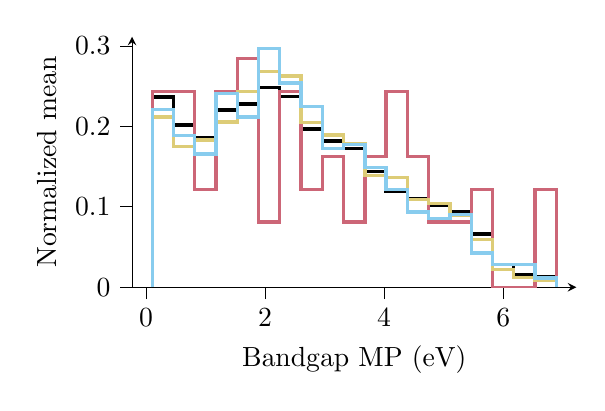
\begin{tikzpicture}

\definecolor{color0}{rgb}{0.8,0.4,0.466666666666667}
\definecolor{color1}{rgb}{0.866666666666667,0.8,0.466666666666667}
\definecolor{color2}{rgb}{0.533333333333333,0.8,0.933333333333333}

\begin{axis}[
height=1.875590092707901in,
legend cell align={left},
legend style={fill opacity=0.8, draw opacity=1, text opacity=1, draw=white!80!black},
tick align=outside,
tick pos=left,
width=2.8444876158848764in,
x grid style={white!69.0196078431373!black},
xlabel={Bandgap MP (eV)},
xmin=-0.234255, xmax=7.229355,
xtick style={color=black},
y grid style={white!69.0196078431373!black},
ylabel={Normalized mean},
ymin=0, ymax=0.311403263332343,
ytick style={color=black}
]
\path [draw=black, very thick]
(axis cs:0.105,0)
--(axis cs:0.105,0.236513148142053)
--(axis cs:0.462110526315789,0.236513148142053)
--(axis cs:0.462110526315789,0.201717735548859)
--(axis cs:0.819221052631579,0.201717735548859)
--(axis cs:0.819221052631579,0.185455961965786)
--(axis cs:1.17633157894737,0.185455961965786)
--(axis cs:1.17633157894737,0.22025137455898)
--(axis cs:1.53344210526316,0.22025137455898)
--(axis cs:1.53344210526316,0.227784402027609)
--(axis cs:1.89055263157895,0.227784402027609)
--(axis cs:1.89055263157895,0.248350762735614)
--(axis cs:2.24766315789474,0.248350762735614)
--(axis cs:2.24766315789474,0.237350151194123)
--(axis cs:2.60477368421053,0.237350151194123)
--(axis cs:2.60477368421053,0.196695717236439)
--(axis cs:2.96188421052632,0.196695717236439)
--(axis cs:2.96188421052632,0.18162966229918)
--(axis cs:3.31899473684211,0.18162966229918)
--(axis cs:3.31899473684211,0.17230305686183)
--(axis cs:3.67610526315789,0.17230305686183)
--(axis cs:3.67610526315789,0.143964524956032)
--(axis cs:4.03321578947368,0.143964524956032)
--(axis cs:4.03321578947368,0.118854433393934)
--(axis cs:4.39032631578947,0.118854433393934)
--(axis cs:4.39032631578947,0.110364831008653)
--(axis cs:4.74743684210526,0.110364831008653)
--(axis cs:4.74743684210526,0.101516513029628)
--(axis cs:5.10454736842105,0.101516513029628)
--(axis cs:5.10454736842105,0.0941030574255792)
--(axis cs:5.46165789473684,0.0941030574255792)
--(axis cs:5.46165789473684,0.066003669248945)
--(axis cs:5.81876842105263,0.066003669248945)
--(axis cs:5.81876842105263,0.0282189600412156)
--(axis cs:6.17587894736842,0.0282189600412156)
--(axis cs:6.17587894736842,0.0159030579893291)
--(axis cs:6.53298947368421,0.0159030579893291)
--(axis cs:6.53298947368421,0.0132724769685379)
--(axis cs:6.8901,0.0132724769685379)
--(axis cs:6.8901,0);

\path [draw=color0, very thick]
(axis cs:0.105,0)
--(axis cs:0.105,0.243500304054985)
--(axis cs:0.462110526315789,0.243500304054985)
--(axis cs:0.462110526315789,0.243500304054985)
--(axis cs:0.819221052631579,0.243500304054985)
--(axis cs:0.819221052631579,0.121750152027492)
--(axis cs:1.17633157894737,0.121750152027492)
--(axis cs:1.17633157894737,0.243500304054985)
--(axis cs:1.53344210526316,0.243500304054985)
--(axis cs:1.53344210526316,0.284083688064149)
--(axis cs:1.89055263157895,0.284083688064149)
--(axis cs:1.89055263157895,0.0811667680183283)
--(axis cs:2.24766315789474,0.0811667680183283)
--(axis cs:2.24766315789474,0.243500304054985)
--(axis cs:2.60477368421053,0.243500304054985)
--(axis cs:2.60477368421053,0.121750152027492)
--(axis cs:2.96188421052632,0.121750152027492)
--(axis cs:2.96188421052632,0.162333536036657)
--(axis cs:3.31899473684211,0.162333536036657)
--(axis cs:3.31899473684211,0.0811667680183284)
--(axis cs:3.67610526315789,0.0811667680183284)
--(axis cs:3.67610526315789,0.162333536036656)
--(axis cs:4.03321578947368,0.162333536036656)
--(axis cs:4.03321578947368,0.243500304054985)
--(axis cs:4.39032631578947,0.243500304054985)
--(axis cs:4.39032631578947,0.162333536036657)
--(axis cs:4.74743684210526,0.162333536036657)
--(axis cs:4.74743684210526,0.0811667680183287)
--(axis cs:5.10454736842105,0.0811667680183287)
--(axis cs:5.10454736842105,0.0811667680183283)
--(axis cs:5.46165789473684,0.0811667680183283)
--(axis cs:5.46165789473684,0.121750152027492)
--(axis cs:5.81876842105263,0.121750152027492)
--(axis cs:5.81876842105263,0)
--(axis cs:6.17587894736842,0)
--(axis cs:6.17587894736842,0)
--(axis cs:6.53298947368421,0)
--(axis cs:6.53298947368421,0.121750152027492)
--(axis cs:6.8901,0.121750152027492)
--(axis cs:6.8901,0);

\path [draw=color1, very thick]
(axis cs:0.105,0)
--(axis cs:0.105,0.211705159535762)
--(axis cs:0.462110526315789,0.211705159535762)
--(axis cs:0.462110526315789,0.1748597187906)
--(axis cs:0.819221052631579,0.1748597187906)
--(axis cs:0.819221052631579,0.18297820573445)
--(axis cs:1.17633157894737,0.18297820573445)
--(axis cs:1.17633157894737,0.205460169578955)
--(axis cs:1.53344210526316,0.205460169578955)
--(axis cs:1.53344210526316,0.242930109319798)
--(axis cs:1.89055263157895,0.242930109319798)
--(axis cs:1.89055263157895,0.267910069147027)
--(axis cs:2.24766315789474,0.267910069147027)
--(axis cs:2.24766315789474,0.262289578185901)
--(axis cs:2.60477368421053,0.262289578185901)
--(axis cs:2.60477368421053,0.204835670583274)
--(axis cs:2.96188421052632,0.204835670583274)
--(axis cs:2.96188421052632,0.189223195691257)
--(axis cs:3.31899473684211,0.189223195691257)
--(axis cs:3.31899473684211,0.178606712764685)
--(axis cs:3.67610526315789,0.178606712764685)
--(axis cs:3.67610526315789,0.138638777041119)
--(axis cs:4.03321578947368,0.138638777041119)
--(axis cs:4.03321578947368,0.136765280054077)
--(axis cs:4.39032631578947,0.136765280054077)
--(axis cs:4.39032631578947,0.108662825248444)
--(axis cs:4.74743684210526,0.108662825248444)
--(axis cs:4.74743684210526,0.10429133227868)
--(axis cs:5.10454736842105,0.10429133227868)
--(axis cs:5.10454736842105,0.0893033563823422)
--(axis cs:5.46165789473684,0.0893033563823422)
--(axis cs:5.46165789473684,0.0593274045896679)
--(axis cs:5.81876842105263,0.0593274045896679)
--(axis cs:5.81876842105263,0.021857464848825)
--(axis cs:6.17587894736842,0.021857464848825)
--(axis cs:6.17587894736842,0.0124899799136143)
--(axis cs:6.53298947368421,0.0124899799136143)
--(axis cs:6.53298947368421,0.00811848694384929)
--(axis cs:6.8901,0.00811848694384929)
--(axis cs:6.8901,0);
\path [draw=color2, very thick]
(axis cs:0.105,0)
--(axis cs:0.105,0.221202002367094)
--(axis cs:0.462110526315789,0.221202002367094)
--(axis cs:0.462110526315789,0.188431335349747)
--(axis cs:0.819221052631579,0.188431335349747)
--(axis cs:0.819221052631579,0.165491868437604)
--(axis cs:1.17633157894737,0.165491868437604)
--(axis cs:1.17633157894737,0.240864402577503)
--(axis cs:1.53344210526316,0.240864402577503)
--(axis cs:1.53344210526316,0.21137080226189)
--(axis cs:1.89055263157895,0.21137080226189)
--(axis cs:1.89055263157895,0.296574536506993)
--(axis cs:2.24766315789474,0.296574536506993)
--(axis cs:2.24766315789474,0.253972669384442)
--(axis cs:2.60477368421053,0.253972669384442)
--(axis cs:2.60477368421053,0.224479069068829)
--(axis cs:2.96188421052632,0.224479069068829)
--(axis cs:2.96188421052632,0.172046001841073)
--(axis cs:3.31899473684211,0.172046001841073)
--(axis cs:3.31899473684211,0.176961601893676)
--(axis cs:3.67610526315789,0.176961601893676)
--(axis cs:3.67610526315789,0.14910653492893)
--(axis cs:4.03321578947368,0.14910653492893)
--(axis cs:4.03321578947368,0.121251467964185)
--(axis cs:4.39032631578947,0.121251467964185)
--(axis cs:4.39032631578947,0.0933964009994398)
--(axis cs:4.74743684210526,0.0933964009994398)
--(axis cs:4.74743684210526,0.0852037342451034)
--(axis cs:5.10454736842105,0.0852037342451034)
--(axis cs:5.10454736842105,0.090119334297705)
--(axis cs:5.46165789473684,0.090119334297705)
--(axis cs:5.46165789473684,0.0426018671225515)
--(axis cs:5.81876842105263,0.0426018671225515)
--(axis cs:5.81876842105263,0.0278550669647452)
--(axis cs:6.17587894736842,0.0278550669647452)
--(axis cs:6.17587894736842,0.0278550669647452)
--(axis cs:6.53298947368421,0.0278550669647452)
--(axis cs:6.53298947368421,0.0114697334560715)
--(axis cs:6.8901,0.0114697334560715)
--(axis cs:6.8901,0);

\end{axis}

\end{tikzpicture}
}
    \subcaption{}
\end{subfigure}
\caption{Number of predicted suitable materials as a function of the (a) standard deviation of the chemical environment of the gaussian symmetric function. Panels (b) crystal fingerprint and (c) OP site fingerprint are related to bond orientational parameters, while (d) shows the band gap referenced to the normalized mean of the entire data set. 
The Ferrenti and extended Ferrenti approaches refer to the left y-axis and the empirical approach to the right. All panels were taken for a $0.75$ cut-off. }
\label{fig:histograms_supp2}
\end{figure}

Figure~\ref{fig:histograms_supp2} shows the number of predicted suitable materials for all approaches (all ML methods in an approach agree to a $0.75$ confidence level) as a function of bond orientational parameters and band gap. 
Panels (a) chemical environment site fingerprint, (b) crystal fingerprint and (c) OP site fingerprint are related to bond orientational parameters, while (d) shows the material band gaps referenced to the normalized mean of the entire data set.  

\newpage 

\bibliography{apssamp}% Produces the bibliography via BibTeX.

\end{document}

